%% abtex2-modelo-trabalho-academico.tex, v-1.9.2 laurocesar
%% Copyright 2012-2014 by abnTeX2 group at http://abntex2.googlecode.com/ 
%%
%% This work may be distributed and/or modified under the
%% conditions of the LaTeX Project Public License, either version 1.3
%% of this license or (at your option) any later version.
%% The latest version of this license is in
%%   http://www.latex-project.org/lppl.txt
%% and version 1.3 or later is part of all distributions of LaTeX
%% version 2005/12/01 or later.
%%
%% This work has the LPPL maintenance status `maintained'.
%% 
%% The Current Maintainer of this work is the abnTeX2 team, led
%% by Lauro César Araujo. Further information are available on 
%% http://abntex2.googlecode.com/
%%
%% This work consists of the files abntex2-modelo-trabalho-academico.tex,
%% abntex2-modelo-include-comandos and abntex2-modelo-references.bib
%%

% ------------------------------------------------------------------------
% ------------------------------------------------------------------------
% abnTeX2: Modelo de Trabalho Academico (tese de doutorado, dissertacao de
% mestrado e trabalhos monograficos em geral) em conformidade com 
% ABNT NBR 14724:2011: Informacao e documentacao - Trabalhos academicos -
% Apresentacao
% ------------------------------------------------------------------------
% ------------------------------------------------------------------------

%-------------------------------------------------------------------------
% Modelo adaptado especificamente para o contexto do PPgSI-EACH-USP por 
% Marcelo Fantinato, com auxílio dos Professores Norton T. Roman, Helton
% H. Bíscaro e Sarajane M. Peres, em 2015, com muitos agradecimentos aos 
% criadores da classe e do modelo base.
%
% 20/06/2017: inclusão de "lista de quadros" com base no especificado em:
% https://github.com/abntex/abntex2/wiki/HowToCriarNovoAmbienteListing,
% de autoria de "Eduardo de Santana Medeiros Alexandre".
%
%-------------------------------------------------------------------------

\documentclass[
	% -- opções da classe memoir --
	12pt,				% tamanho da fonte
	% openright,			% capítulos começam em pág ímpar (insere página vazia caso preciso)
	oneside,			% para impressão apenas no anverso (apenas frente). Oposto a twoside
	a4paper,			% tamanho do papel. 
	% -- opções da classe abntex2 --
	%chapter=TITLE,		% títulos de capítulos convertidos em letras maiúsculas
	%section=TITLE,		% títulos de seções convertidos em letras maiúsculas
	%subsection=TITLE,	% títulos de subseções convertidos em letras maiúsculas
	%subsubsection=TITLE,% títulos de subsubseções convertidos em letras maiúsculas
	% -- opções do pacote babel --
	english,			% idioma adicional para hifenização
	%french,				% idioma adicional para hifenização
	%spanish,			% idioma adicional para hifenização
	brazil				% o último idioma é o principal do documento
	]{abntex2ppgsi}

% ---
% Pacotes básicos 
% ---
% \usepackage{lmodern}			% Usa a fonte Latin Modern			
% \usepackage[T1]{fontenc}		% Selecao de codigos de fonte.
\usepackage[utf8]{inputenc}		% Codificacao do documento (conversão automática dos acentos)
\usepackage{lastpage}			% Usado pela Ficha catalográfica
\usepackage{indentfirst}		% Indenta o primeiro parágrafo de cada seção.
\usepackage{color}				% Controle das cores
\usepackage{graphicx}			% Inclusão de gráficos
\usepackage{microtype} 			% para melhorias de justificação
\usepackage{pdfpages}     %para incluir pdf
\usepackage{algorithm}			%para ilustrações do tipo algoritmo
\usepackage{mdwlist}			%para itens com espaço padrão da abnt
\usepackage[noend]{algpseudocode}			%para ilustrações do tipo algoritmo


\usepackage{lscape}
\usepackage{longtable}
\usepackage{setspace}

\hyphenation{pro-ces-sa-men-to}

% ---
% Pacotes adicionais, usados apenas no âmbito do Modelo Canônico do abnteX2
% ---
\usepackage{lipsum}				% para geração de dummy text
% ---

% ---
% Pacotes de citações
% ---
\usepackage{hyperref}
\usepackage[brazilian,hyperpageref]{backref}	 % Paginas com as citações na bibl
\usepackage[alf,abnt-etal-list=0,abnt-etal-text=it]{abntex2cite}	% Citações padrão ABNT

% --- 
% CONFIGURAÇÕES DE PACOTES
% --- 

% ---
% Configurações do pacote backref
% Usado sem a opção hyperpageref de backref
\renewcommand{\backrefpagesname}{Citado na(s) página(s):~}
% Texto padrão antes do número das páginas
\renewcommand{\backref}{}
% Define os textos da citação
\renewcommand*{\backrefalt}[4]{
	\ifcase #1 %
		Nenhuma citação no texto.%
	\or
		Citado na página #2.%
	\else
		Citado #1 vezes nas páginas #2.%
	\fi}%
% ---

% ---
% Informações de dados para CAPA e FOLHA DE ROSTO
% ---

%-------------------------------------------------------------------------
% Comentário adicional do PPgSI - Informações sobre o ``instituicao'':
%
% Não mexer. Deixar exatamente como está.
%
%-------------------------------------------------------------------------
\instituicao{
	UNIVERSIDADE DE SÃO PAULO
	\par
	ESCOLA DE ARTES, CIÊNCIAS E HUMANIDADES
	\par
	PROGRAMA DE PÓS-GRADUAÇÃO EM SISTEMAS DE INFORMAÇÃO}

%-------------------------------------------------------------------------
% Comentário adicional do PPgSI - Informações sobre o ``título'':
%
% Em maiúscula apenas a primeira letra da sentença (do título), exceto 
% nomes próprios, geográficos, institucionais ou Programas ou Projetos ou 
% siglas, os quais podem ter letras em maiúscula também.
%
% O subtítulo do trabalho é opcional.
% Sem ponto final.
%
% Atenção: o título da Dissertação/Tese na versão corrigida não pode mudar. 
% Ele deve ser idêntico ao da versão original.
%
%-------------------------------------------------------------------------
\titulo{Classificação automática de espécies de abelhas por meio da morfologia de suas asas capturadas em imagens digitais utilizando rede neural convolucional}

%-------------------------------------------------------------------------
% Comentário adicional do PPgSI - Informações sobre o ``autor'':
%
% Todas as letras em maiúsculas.
% Nome completo.
% Sem ponto final.
%-------------------------------------------------------------------------
\autor{\uppercase{Danilo Souza de Assunção}}

%-------------------------------------------------------------------------
% Comentário adicional do PPgSI - Informações sobre o ``local'':
%
% Não incluir o ``estado''.
% Sem ponto final.
%-------------------------------------------------------------------------
\local{São Paulo}

%-------------------------------------------------------------------------
% Comentário adicional do PPgSI - Informações sobre a ``data'':
%
% Colocar o ano do depósito (ou seja, o ano da entrega) da respectiva 
% versão, seja ela a versão original (para a defesa) seja ela a versão 
% corrigida (depois da aprovação na defesa). 
%
% Atenção: Se a versão original for depositada no final do ano e a versão 
% corrigida for entregue no ano seguinte, o ano precisa ser atualizado no 
% caso da versão corrigida. 
% Cuidado, pois o ano da ``capa externa'' também precisa ser atualizado 
% nesse caso.
%
% Não incluir o dia, nem o mês.
% Sem ponto final.
%-------------------------------------------------------------------------
\data{2021}

%-------------------------------------------------------------------------
% Comentário adicional do PPgSI - Informações sobre o ``Orientador'':
%
% Se for uma professora, trocar por ``Profa. Dra.''
% Nome completo.
% Sem ponto final.
%-------------------------------------------------------------------------
\orientador{Prof. Dr. Helton Hideraldo Biscaro}

%-------------------------------------------------------------------------
% Comentário adicional do PPgSI - Informações sobre o ``Coorientador'':
%
% Opcional. Incluir apenas se houver co-orientador formal, de acordo com o 
% Regulamento do Programa.
%
% Se for uma professora, trocar por ``Profa. Dra.''
% Nome completo.
% Sem ponto final.
%-------------------------------------------------------------------------
\coorientador{Prof. Dr. Luciano Antonio Digiampietri}

\tipotrabalho{Dissertação (Mestrado)}

\preambulo{
%-------------------------------------------------------------------------
% Comentário adicional do PPgSI - Informações sobre o texto ``Versão 
% original'':
%
% Não usar para Qualificação.
% Não usar para versão corrigida de Dissertação/Tese.
%
%-------------------------------------------------------------------------
Versão original \newline \newline \newline 
%-------------------------------------------------------------------------
% Comentário adicional do PPgSI - Informações sobre o ``texto principal do
% preambulo'':
%
% Para Doutorado, trocar por: Tese apresentada à Escola de Artes, Ciências e Humanidades da Universidade de São Paulo para obtenção do título de Doutor (ou Doutora) em Ciências pelo Programa de Pós-graduação em Sistemas de Informação. 
%
% Para Qualificação, trocar por: Projeto de pesquisa para exame de qualificação apresentado à Escola de Artes, Ciências e Humanidades da Universidade de São Paulo como parte dos requisitos para obtenção do título de Mestre (ou Doutor ou Doutora) em Ciências pelo Programa de Pós-graduação em Sistemas de Informação.
%
%-------------------------------------------------------------------------
Dissertação apresentada à Escola de Artes, Ciências e Humanidades da Universidade de São Paulo para obtenção do título de Mestre em Ciências pelo Programa de Pós-graduação em Sistemas de Informação.
%
\newline \newline Área de concentração: Metodologia e Técnicas da Computação
%-------------------------------------------------------------------------
% Comentário adicional do PPgSI - Informações sobre o texto da ``Versão 
% corrigida'':
%
% Não usar para Qualificação.
% Não usar para versão original de Dissertação/Tese.
% 
% Substituir ``xx de xxxxxxxxxxxxxxx de xxxx'' pela ``data da defesa''.
%
%-------------------------------------------------------------------------
\newline \newline \newline Versão corrigida contendo as alterações solicitadas pela comissão julgadora em xx de xxxxxxxxxxxxxxx de xxxx. A versão original encontra-se em acervo reservado na Biblioteca da EACH-USP e na Biblioteca Digital de Teses e Dissertações da USP (BDTD), de acordo com a Resolução CoPGr 6018, de 13 de outubro de 2011.}
% ---


% ---
% Configurações de aparência do PDF final

% alterando o aspecto da cor azul
\definecolor{blue}{RGB}{41,5,195}

% informações do PDF
\makeatletter
\hypersetup{
     	%pagebackref=true,
		pdftitle={\@title}, 
		pdfauthor={\@author},
    	pdfsubject={\imprimirpreambulo},
	    pdfcreator={laTeX com abnTeX2 adaptado para o PPgSI-EACH-USP},
		pdfkeywords={abnt}{latex}{abntex}{abntex2ppgsi}{qualificação de mestrado}{dissertação de mestrado}{qualificação de doutorado}{tese de doutorado}{ppgsi}, 
		colorlinks=true,       		% false: boxed links; true: colored links
    	linkcolor=blue,          	% color of internal links
    	citecolor=blue,        		% color of links to bibliography
    	filecolor=magenta,      		% color of file links
		urlcolor=blue,
		bookmarksdepth=4
}
\makeatother
% --- 

% --- 
% Espaçamentos entre linhas e parágrafos 
% --- 

% O tamanho do parágrafo é dado por:
\setlength{\parindent}{1.25cm}

% Controle do espaçamento entre um parágrafo e outro:
\setlength{\parskip}{0cm}  % tente também \onelineskip
\renewcommand{\baselinestretch}{1.5}

% ---
% compila o indice
% ---
\makeindex
% ---

	% Controlar linhas orfas e viuvas
  \clubpenalty10000
  \widowpenalty10000
  \displaywidowpenalty10000

% ----
% Início do documento
% ----
\begin{document}

% Retira espaço extra obsoleto entre as frases.
\frenchspacing 

% ----------------------------------------------------------
% ELEMENTOS PRÉ-TEXTUAIS
% ----------------------------------------------------------
% \pretextual

% ---
% Capa
% ---
%-------------------------------------------------------------------------
% Comentário adicional do PPgSI - Informações sobre a ``capa'':
%
% Esta é a ``capa'' principal/oficial do trabalho, a ser impressa apenas 
% para os casos de encadernação simples (ou seja, em ``espiral'' com 
% plástico na frente).
% 
% Não imprimir esta ``capa'' quando houver ``capa dura'' ou ``capa brochura'' 
% em que estas mesmas informações já estão presentes nela.
%
%-------------------------------------------------------------------------
\imprimircapa
% ---

% ---
% Folha de rosto
% (o * indica que haverá a ficha bibliográfica)
% ---
\imprimirfolhaderosto*
% ---

% ---
% Inserir a autorização para reprodução e ficha bibliografica
% ---

%-------------------------------------------------------------------------
% Comentário adicional do PPgSI - Informações sobre o texto da 
% ``autorização para reprodução e ficha bibliografica'':
%
% Página a ser usada apenas para Dissertação/Tese (tanto na versão original 
% quanto na versão corrigida).
%
% Solicitar a ficha catalográfica na Biblioteca da EACH. 
% Duas versões devem ser solicitadas, em dois momentos distintos: uma vez 
% para a versão original, e depois outra atualizada para a versão 
% corrigida.
%
% Atenção: esta página de ``autorização para reprodução e ficha 
% catalográfica'' deve ser impressa obrigatoriamente no verso da folha de 
% rosto.
%
% Não usar esta página para Qualificação.
%
% Substitua o arquivo ``fig_ficha_catalografica.pdf'' abaixo referenciado 
% pelo PDF elaborado pela Biblioteca
%
%-------------------------------------------------------------------------
\begin{fichacatalografica}
    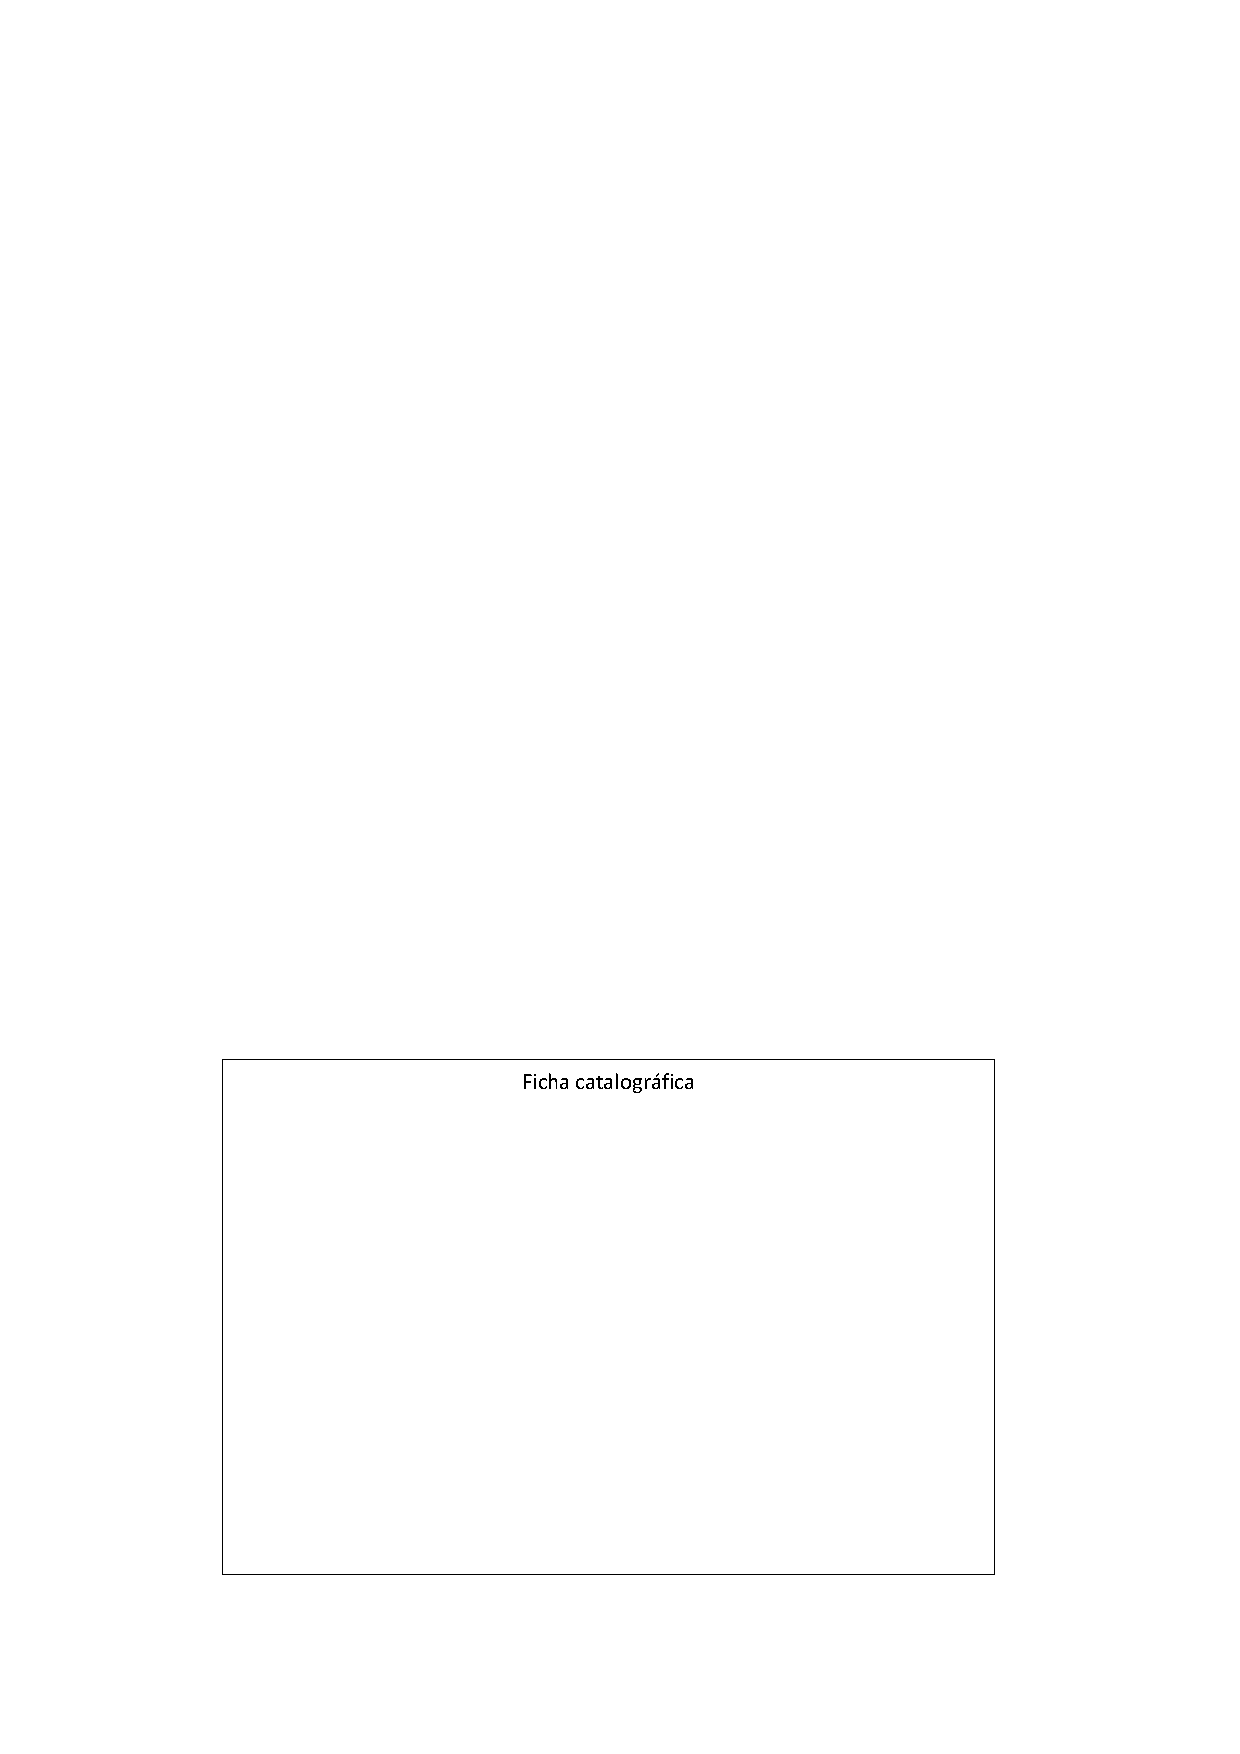
\includepdf{fig_ficha_catalografica.pdf}
\end{fichacatalografica}

% ---
% Inserir errata
% ---
%-------------------------------------------------------------------------
% Comentário adicional do PPgSI - Informações sobre ``Errata'':
%
% Usar esta página de errata apenas em casos de excepcionais, e apenas 
% para a versão corrigida da Dissertação/Tese. Por exemplo, quando depois de
% já depositada e publicada a versão corrigida, ainda assim verifica-se
% a necessidade de alguma correção adicional.
%
% Se precisar usar esta página, busque a forma correta (o modelo correto) 
% para fazê-lo, de acordo com a norma ABNT.
%
% Não usar esta página para versão original de Dissertação/Tese.
% Não usar esta página para Qualificação.
%
%-------------------------------------------------------------------------
\begin{errata}
Elemento opcional para versão corrigida, depois de depositada.
\end{errata}
% ---

% ---
% Inserir folha de aprovação
% ---

\begin{folhadeaprovacao}
%-------------------------------------------------------------------------
% Comentário adicional do PPgSI - Informações sobre ``Folha da aprovação'':
%
% Página a ser usada apenas para Dissertação/Tese.
%
% Não usar esta página para Qualificação.
%
% Substituir ``Fulano de Tal'' pelo nome completo do autor do trabalho, com 
% apenas as iniciais em maiúsculo.
%
% Substituir ``___ de ______________ de ______'' por: 
%     - Para versão original de Dissertação/Tese: deixar em branco, pois a data 
%       pode mudar, mesmo que ela já esteja prevista.
%     - Para versão corrigida de Dissertação/Tese: usar a data em que a defesa 
%       efetivamente ocorreu.
%
% Para Tese de Doutorado: trocar "Dissertação" por "Tese".
%-------------------------------------------------------------------------
\noindent Dissertação de autoria de Fulano de Tal, sob o título \textbf{``\imprimirtitulo''}, apresentada à Escola de Artes, Ciências e Humanidades da Universidade de São Paulo, para obtenção do título de Mestre em Ciências pelo Programa de Pós-graduação em Sistemas de Informação, na área de concentração Metodologia e Técnicas da Computação, aprovada em \rule{0.85cm}{0.5pt} de \rule{3.5cm}{0.5pt} de \rule{1.25cm}{0.5pt} pela comissão julgadora constituída pelos doutores:

\vspace*{3cm}

\begin{center}
%-------------------------------------------------------------------------
% Comentário adicional do PPgSI - Informações sobre ``assinaturas'':
%
% Para versão original de Dissertação/Tese: deixar em 
% branco (ou seja, assim como está abaixo), pois os membros da banca podem
% mudar, mesmo que eles já estejam previstos.
% 
% Para versão corrigida de Dissertação/Tese: usar os dados dos examinadores que 
% efetivamente participaram da defesa. 
% 
% Para versão corrigida de Dissertação/Tese: em caso de ``professora'', trocar 
% por ``Profa. Dra.'' 
% 
% Para versão corrigida de Dissertação/Tese: ao colocar os nomes dos 
% examinadores, usar seus nomes completos, exatamente conforme constam em 
% seus Currículos Lattes
% 
% Para a versão corrigida de Dissertação/Tese: remova o texto “Instituição: ”, 
% ou seja, coloque apenas/diretamente o nome da instituição, por exemplo 
% "Universidade de São Paulo" ou "Universidade Estadual de Campinas".
%
% Não abreviar os nomes das instituições.
%
% Verifique quantos membros há em sua banca, de acordo com o seu regulamento, 
% especificamente para o caso de Dissertação de Mestrado ou Tese de Doutorado, 
% e use o número correto de espaços para assinaturas.
%
%-------------------------------------------------------------------------

\assinatura{Prof. Dr. \\ Instituição \\ Presidente}

\assinatura{Prof. Dr. \\ Instituição}

\assinatura{Prof. Dr. \\ Instituição}

\assinatura{Prof. Dr. \\ Instituição}    % Incluir para bancas de tese de doutorado

\assinatura{Prof. Dr. \\ Instituição}    % Incluir para bancas de tese de doutorado

\end{center}
  
\end{folhadeaprovacao}
% ---

% ---
% Dedicatória
% ---
%-------------------------------------------------------------------------
% Comentário adicional do PPgSI - Informações sobre ``Dedicatória'': 
%
% Opcional para Dissertação/Tese.
% Não sugerido para Qualificação.
% 
%-------------------------------------------------------------------------
\begin{dedicatoria}
   \vspace*{\fill}
   \centering
   \noindent
   \textit{Escreva aqui sua dedicatória, se desejar, ou remova esta página...} 
	 \vspace*{\fill}
\end{dedicatoria}
% ---

% ---
% Agradecimentos
% ---
%-------------------------------------------------------------------------
% Comentário adicional do PPgSI - Informações sobre ``Agradecimentos'': 
%
% Opcional para Dissertação/Tese.
% Não sugerido para Qualificação.
% 
% 
% Financiamentos recebidos durante o projeto de mestrado/doutorado, vindos de qualquer 
% agência de fomento, devem ser mencionados na seção de agradecimentos da dissertação/tese. 
% Isso se aplica não apenas a bolsas de estudo, mas a qualquer tipo de financiamento, 
% tais como para apoio a participação em eventos, compra de materiais, traduções etc. 
% Especificamente para financiamento da Capes, siga as instruções contidas na portaria 
% 206, de 4/set/2018; para outras agências de fomento, procure as regras apropriadas.
%
% Portaria Capes 206, de 4/set/2018: 
% http://ppgsi.each.usp.br/arquivos/Portaria_0783227_Portaria_CAPES_DOU___206_de_2018.pdf 
%
%
%-------------------------------------------------------------------------
\begin{agradecimentos}
Texto de exemplo, texto de exemplo, texto de exemplo, texto de exemplo, texto de exemplo, texto de exemplo, texto de exemplo, texto de exemplo, texto de exemplo, texto de exemplo, texto de exemplo, texto de exemplo, texto de exemplo, texto de exemplo, texto de exemplo, texto de exemplo, texto de exemplo, texto de exemplo, texto de exemplo, texto de exemplo, texto de exemplo, texto de exemplo.

Texto de exemplo, texto de exemplo, texto de exemplo, texto de exemplo, texto de exemplo, texto de exemplo, texto de exemplo, texto de exemplo, texto de exemplo, texto de exemplo, texto de exemplo, texto de exemplo, texto de exemplo, texto de exemplo, texto de exemplo, texto de exemplo, texto de exemplo, texto de exemplo, texto de exemplo, texto de exemplo, texto de exemplo, texto de exemplo.

Texto de exemplo, texto de exemplo, texto de exemplo, texto de exemplo, texto de exemplo, texto de exemplo, texto de exemplo, texto de exemplo, texto de exemplo, texto de exemplo, texto de exemplo, texto de exemplo, texto de exemplo, texto de exemplo, texto de exemplo, texto de exemplo, texto de exemplo, texto de exemplo, texto de exemplo, texto de exemplo, texto de exemplo, texto de exemplo.

Texto de exemplo, texto de exemplo, texto de exemplo, texto de exemplo, texto de exemplo, texto de exemplo, texto de exemplo, texto de exemplo, texto de exemplo, texto de exemplo, texto de exemplo, texto de exemplo, texto de exemplo, texto de exemplo, texto de exemplo, texto de exemplo, texto de exemplo, texto de exemplo, texto de exemplo, texto de exemplo, texto de exemplo, texto de exemplo.

Texto de exemplo, texto de exemplo, texto de exemplo, texto de exemplo, texto de exemplo, texto de exemplo, texto de exemplo, texto de exemplo, texto de exemplo, texto de exemplo, texto de exemplo, texto de exemplo, texto de exemplo, texto de exemplo, texto de exemplo, texto de exemplo, texto de exemplo, texto de exemplo, texto de exemplo, texto de exemplo, texto de exemplo, texto de exemplo.
\end{agradecimentos}
% ---

% ---
% Epígrafe
% ---
%-------------------------------------------------------------------------
% Comentário adicional do PPgSI - Informações sobre ``Epígrafe'': 
%
% Opcional para Dissertação/Tese.
% Não sugerido para Qualificação.
% 
%-------------------------------------------------------------------------
\begin{epigrafe}
    \vspace*{\fill}
	\begin{flushright}
		\textit{``Eu acredito muito na sorte. E tenho constatado que, quanto mais duro eu trabalho, mais sorte eu tenho.''\\
		(Thomas Jefferson)}
	\end{flushright}
\end{epigrafe}
% ---

% ---
% RESUMOS
% ---

% resumo em português
\setlength{\absparsep}{18pt} % ajusta o espaçamento dos parágrafos do resumo
\begin{resumo}

%-------------------------------------------------------------------------
% Comentário adicional do PPgSI - Informações sobre ``referência'':
% 
% Troque os seguintes campos pelos dados de sua Dissertação/Tese (mantendo a 
% formatação e pontuação):
%   - SOBRENOME
%   - Nome1
%   - Nome2
%   - Nome3
%   - Título do trabalho: subtítulo do trabalho
%   - AnoDeDefesa
%
% Mantenha todas as demais informações exatamente como estão.
% 
% [Não usar essas informações de ``referência'' para Qualificação]
%
% Para Tese de Doutorado: trocar "Dissertação (Mestrado em Ciências)" por "Tese (Doutorado em Ciências)".
%-------------------------------------------------------------------------
\begin{flushleft}
SOBRENOME, Nome1 Nome2 Nome3. \textbf{Título do trabalho}: subtítulo do trabalho. \imprimirdata. \pageref{LastPage} f. Dissertação (Mestrado em Ciências) – Escola de Artes, Ciências e Humanidades, Universidade de São Paulo, São Paulo, AnoDeDefesa.
\end{flushleft}

Escreva aqui o texto do seu resumo... (redigido em parágrafo único, no máximo em uma página, contendo no ``máximo 500 palavras'', e apresentando um resumo de todos o seu trabalho, incluindo objetivos, metodologia, resultados e conclusões; não inclua apenas a contextualização até chegar nos objetivos, é importante fazer um resumo de todos os capítulos do texto, até chegar à conclusão). Texto de exemplo, texto de exemplo, texto de exemplo, texto de exemplo, texto de exemplo, texto de exemplo, texto de exemplo, texto de exemplo, texto de exemplo, texto de exemplo, texto de exemplo, texto de exemplo, texto de exemplo, texto de exemplo, texto de exemplo, texto de exemplo, texto de exemplo, texto de exemplo, texto de exemplo, texto de exemplo, texto de exemplo, texto de exemplo.

Palavras-chaves: Palavra1. Palavra2. Palavra3. etc.
\end{resumo}

% resumo em inglês
%-------------------------------------------------------------------------
% Comentário adicional do PPgSI - Informações sobre ``resumo em inglês''
% 
% Caso a Qualificação ou a Dissertação/Tese inteira seja elaborada no idioma inglês, 
% então o ``Abstract'' vem antes do ``Resumo''.
% 
%-------------------------------------------------------------------------
\begin{resumo}[Abstract]
\begin{otherlanguage*}{english}

%-------------------------------------------------------------------------
% Comentário adicional do PPgSI - Informações sobre ``referência em inglês''
% 
% Troque os seguintes campos pelos dados de sua Dissertação/Tese (mantendo a 
% formatação e pontuação):
%     - SURNAME
%     - FirstName1
%     - MiddleName1
%     - MiddleName2
%     - Work title: work subtitle
%     - DefenseYear (Ano de Defesa)
%
% Mantenha todas as demais informações exatamente como estão.
%
% [Não usar essas informações de ``referência'' para Qualificação]
%
%-------------------------------------------------------------------------
\begin{flushleft}
SURNAME, FirstName MiddleName1 MiddleName2. \textbf{Work title}: work subtitle. \imprimirdata. \pageref{LastPage} p. Dissertation (Master of Science) – School of Arts, Sciences and Humanities, University of São Paulo, São Paulo, DefenseYear. 
\end{flushleft}

Write here the English version of your ``Resumo''. Example text, example text, example text, example text, example text, example text, example text, example text, example text, example text, example text, example text, example text, example text, example text, example text, example text, example text, example text, example text, example text, example text, example text, example text, example text, example text, example text, example text, example text, example text, example text, example text, example text, example text, example text, example text, example text, example text, example text, example text, example text, example text, example text, example text, example text, example text, example text.

Keywords: Keyword1. Keyword2. Keyword3. etc.
\end{otherlanguage*}
\end{resumo}

% ---
% ---
% inserir lista de figuras
% ---
\pdfbookmark[0]{\listfigurename}{lof}
\listoffigures*
\cleardoublepage
% ---

% ---
% inserir lista de algoritmos
% ---
\pdfbookmark[0]{\listalgorithmname}{loa}
\listofalgorithms
\cleardoublepage

% ---
% inserir lista de quadros
% ---
\pdfbookmark[0]{\listofquadrosname}{loq}
\listofquadros*
\cleardoublepage


% ---
% inserir lista de tabelas
% ---
\pdfbookmark[0]{\listtablename}{lot}
\listoftables*
\cleardoublepage
% ---

% ---
% inserir lista de abreviaturas e siglas
% ---
%-------------------------------------------------------------------------
% Comentário adicional do PPgSI - Informações sobre ``Lista de abreviaturas 
% e siglas'': 
%
% Opcional.
% Uma vez que se deseja usar, é necessário manter padrão e consistência no
% trabalho inteiro.
% Se usar: inserir em ordem alfabética.
%
%-------------------------------------------------------------------------
\begin{siglas}
  \item[Sigla/abreviatura 1] Definição da sigla ou da abreviatura por extenso
  \item[Sigla/abreviatura 2] Definição da sigla ou da abreviatura por extenso
  \item[Sigla/abreviatura 3] Definição da sigla ou da abreviatura por extenso
  \item[Sigla/abreviatura 4] Definição da sigla ou da abreviatura por extenso
  \item[Sigla/abreviatura 5] Definição da sigla ou da abreviatura por extenso
  \item[Sigla/abreviatura 6] Definição da sigla ou da abreviatura por extenso
  \item[Sigla/abreviatura 7] Definição da sigla ou da abreviatura por extenso
  \item[Sigla/abreviatura 8] Definição da sigla ou da abreviatura por extenso
  \item[Sigla/abreviatura 9] Definição da sigla ou da abreviatura por extenso
  \item[Sigla/abreviatura 10] Definição da sigla ou da abreviatura por extenso
\end{siglas}
% ---

% ---
% inserir lista de símbolos
% ---
%-------------------------------------------------------------------------
% Comentário adicional do PPgSI - Informações sobre ``Lista de símbolos'': 
%
% Opcional.
% Uma vez que se deseja usar, é necessário manter padrão e consistência no
% trabalho inteiro.
% Se usar: inserir na ordem em que aparece no texto.
% 
%-------------------------------------------------------------------------
\begin{simbolos}
  \item[$ \Gamma $] Letra grega Gama
  \item[$ \Lambda $] Lambda
  \item[$ \zeta $] Letra grega minúscula zeta
  \item[$ \in $] Pertence
\end{simbolos}
% ---

% ---
% inserir o sumario
% ---
\pdfbookmark[0]{\contentsname}{toc}
\tableofcontents*
\cleardoublepage
% ---



% ----------------------------------------------------------
% ELEMENTOS TEXTUAIS
% ----------------------------------------------------------
\textual



%-------------------------------------------------------------------------
% Comentário adicional do PPgSI - Informações sobre ``títulos de seções''
% 
% Para todos os títulos (seções, subseções, tabelas, ilustrações, etc.):
%
% Em maiúscula apenas a primeira letra da sentença (do título), exceto 
% nomes próprios, geográficos, institucionais ou Programas ou Projetos ou
% siglas, os quais podem ter letras em maiúscula também.
%
%-------------------------------------------------------------------------
\chapter{Introdução}
As plantações alimentícias possuem uma elevada dependência  em relação as abelhas, cuja a responsabilidade de polinização se encontra por volta de 70\% \cite{drauschke2007reliable}, ou seja, as abelhas economizam um serviço no qual custariam cerca de 65 bilhões de dólares anualmente \cite{pimentel1997economic}. Sendo elas também responsáveis por um papel de extrema valia para a natureza, onde a preservação de ecossistemas terrestres em conjunto de seu relacionamento com as abelhas \cite{lawton1998daily}. 

Diante disso, o processo de classificação de espécies de abelhas acaba por ser um importante sistema para a sua preservação, por obter informações detalhadas e possibilitando estabelecer estratégias mais precisas de conservação de uma determinada espécie e também para uma localidade especifica \cite{goulson2015bee}. 

A realização automática da análise visual da morfologia das abelhas se convêm devido as despesas necessárias nos processos de identificação manual, e para esta análise morfológica, os conjuntos de características extraídos a partir das asas têm se mostrado uma maneira eficiente para a identificação das espécies utilizando métodos estatísticos \cite{francoy2008identification}.


\section{Problema de pesquisa}
 
Texto de exemplo, texto de exemplo, texto de exemplo, texto de exemplo, texto de exemplo, texto de exemplo, texto de exemplo, texto de exemplo, texto de exemplo, texto de exemplo, texto de exemplo, texto de exemplo, texto de exemplo, texto de exemplo, texto de exemplo, texto de exemplo, texto de exemplo, texto de exemplo, texto de exemplo, texto de exemplo, texto de exemplo, texto de exemplo, texto de exemplo.

A figura \ref{fig:figura-exemplo2} é um exemplo de como apresentar ilustrações de acordo com essa norma. Qualquer outra ilustração deve ser apresentada de forma similar, mudando apenas o prefixo do título e a numeração. Veja mais detalhes no anexo \ref{anexoA} deste documento.

A figura \ref{fig:figura-exemplo2} também apresenta um exemplo de como incluir em ``Fonte:'' uma citação para um trabalho já publicado, seja do próprio autor ou de outro autor. Nesse caso, use sempre o ``citeonline'', para o ano ficar separado do nome do autor, entre parênteses. Use sempre o ``citeonline'' inclusive para referenciar um trabalho do próprio autor, onde a imagem, tabela ou outro elemento já foi publicado. Se for do próprio autor, mas ainda não publicado, então seguir o exemplo apresentado na figura \ref{fig:figura-exemplo1}.

\begin{figure}[htbp]
	\centering
  \caption{Exemplo de título de ilustração do tipo figura, que pode ser maior para apresentar mais explicações sobre o conteúdo da figura, se for o caso; e com exemplo de citação a um trabalho já publicado, seja do próprio autor ou de outro autor}
		
\includegraphics{figura-exemplo.png}
	\label{fig:figura-exemplo2}
  \source{\citeonline{teste3}}
\end{figure}

Texto de exemplo, texto de exemplo, texto de exemplo, texto de exemplo, texto de exemplo, texto de exemplo, texto de exemplo, texto de exemplo, texto de exemplo, texto de exemplo, texto de exemplo, texto de exemplo, texto de exemplo, texto de exemplo, texto de exemplo, texto de exemplo, texto de exemplo, texto de exemplo, texto de exemplo, texto de exemplo, texto de exemplo, texto de exemplo, texto de exemplo.

\subsection{Uma seção terciária}

Texto de exemplo, texto de exemplo, texto de exemplo, texto de exemplo, texto de exemplo, texto de exemplo, texto de exemplo, texto de exemplo, texto de exemplo, texto de exemplo, texto de exemplo, texto de exemplo, texto de exemplo, texto de exemplo, texto de exemplo, texto de exemplo, texto de exemplo, texto de exemplo, texto de exemplo, texto de exemplo, texto de exemplo, texto de exemplo, texto de exemplo.

A tabela \ref{tab:ExemploDeTabela2} é outro exemplo de como apresentar tabelas de acordo com essa norma. Veja mais detalhes no anexo \ref{anexoA} deste documento.

\begin{table}[htbp]
	\centering
	\caption{Exemplo de título de tabela, que pode ser maior para apresentar mais explicações sobre o conteúdo da tabela, se for o caso}
		\begin{tabular}{p{1.2in} p{1.2in} p{1.2in} p{1.2in} } \hline
		
		Cabeçalho 1	& Cabeçalho 2	& Cabeçalho 3	& Cabeçalho 4 \\ \hline
		Texto	& número & número	& número \\ 
		Texto	& número & número	& número \\ 
		Texto	& número & número	& número \\ 
		Texto	& número & número	& número \\ 
		Texto	& número & número	& número \\ \hline
			
		\end{tabular}
	\label{tab:ExemploDeTabela2}
  \source{Marcelo Fantinato, 2015}
\end{table}

\subsection{Outra seção terciária}

Texto de exemplo, texto de exemplo, texto de exemplo, texto de exemplo, texto de exemplo, texto de exemplo, texto de exemplo, texto de exemplo, texto de exemplo, texto de exemplo, texto de exemplo, texto de exemplo, texto de exemplo, texto de exemplo, texto de exemplo, texto de exemplo, texto de exemplo, texto de exemplo, texto de exemplo, texto de exemplo, texto de exemplo, texto de exemplo, texto de exemplo.

Texto de exemplo, texto de exemplo, texto de exemplo, texto de exemplo, texto de exemplo, texto de exemplo, texto de exemplo, texto de exemplo, texto de exemplo, texto de exemplo, texto de exemplo, texto de exemplo, texto de exemplo, texto de exemplo, texto de exemplo, texto de exemplo, texto de exemplo, texto de exemplo, texto de exemplo, texto de exemplo, texto de exemplo, texto de exemplo, texto de exemplo.

A figura \ref{fig:figura-exemplo3} é um exemplo de como apresentar ilustrações de acordo com essa norma. Qualquer outra ilustração deve ser apresentada de forma similar, mudando apenas o prefixo do título e a numeração. Veja mais detalhes no anexo \ref{anexoA} deste documento.

\begin{figure}[htbp]
	\centering
	\caption{Exemplo de título de ilustração do tipo figura}
		
\includegraphics{figura-exemplo.png}
	\label{fig:figura-exemplo3}
  \source{Marcelo Fantinato, 2015}
\end{figure}

O quadro \ref{qua:ExemploDeQuadro2} é mais um exemplo de como apresentar quadros de acordo com essa norma. Veja mais detalhes no anexo \ref{anexoA} deste documento.

\begin{quadro}[H]
	\centering
	\caption{Exemplo de título de quadro}
	\begin{tabular}{|p{1in} | p{1in} | p{1in} | p{1in} |} \hline
		
		Cabeçalho 1	& Cabeçalho 2	& Cabeçalho 3	& Cabeçalho 4 \\ \hline
		Texto	& texto & texto	& texto \\ \hline
		Texto	& texto & texto	& texto \\ \hline
		Texto	& texto & texto	& texto \\ \hline
		Texto	& texto & texto	& texto \\ \hline
		Texto	& texto & texto	& texto \\ \hline
		
	\end{tabular}
	\label{qua:ExemploDeQuadro2}
	\source{Marcelo Fantinato, 2015}
\end{quadro}

O quadro \ref{qua:ExemploDeQuadro3} é mais um exemplo de como apresentar quadros de acordo com essa norma. Veja mais detalhes no anexo \ref{anexoA} deste documento.

\begin{quadro}[H]
	\centering
	\caption{Exemplo de título de quadro}
	\begin{tabular}{|p{1in} | p{1in} | p{1in} | p{1in} |} \hline
		
		Cabeçalho 1	& Cabeçalho 2	& Cabeçalho 3	& Cabeçalho 4 \\ \hline
		Texto	& texto & texto	& texto \\ \hline
		Texto	& texto & texto	& texto \\ \hline
		Texto	& texto & texto	& texto \\ \hline
		Texto	& texto & texto	& texto \\ \hline
		Texto	& texto & texto	& texto \\ \hline
		
	\end{tabular}
	\label{qua:ExemploDeQuadro3}
	\source{Marcelo Fantinato, 2015}
\end{quadro}

\subsection{Mais uma seção terciária}

Texto de exemplo, texto de exemplo, texto de exemplo, texto de exemplo, texto de exemplo, texto de exemplo, texto de exemplo, texto de exemplo, texto de exemplo, texto de exemplo, texto de exemplo, texto de exemplo, texto de exemplo, texto de exemplo, texto de exemplo, texto de exemplo, texto de exemplo, texto de exemplo, texto de exemplo, texto de exemplo, texto de exemplo, texto de exemplo, texto de exemplo.

A tabela \ref{tab:ExemploDeTabela3} é um exemplo de como apresentar tabelas de acordo com essa norma. Veja mais detalhes no anexo \ref{anexoA} deste documento.

\begin{table}[htbp]
	\centering
	\caption{Exemplo de título de tabela}
		\begin{tabular}{p{0.85in} p{0.85in} p{0.85in} p{0.85in} } \hline
		
		Cabeçalho 1	& Cabeçalho 2	& Cabeçalho 3	& Cabeçalho 4 \\ \hline
		Texto	& número & número	& número \\ 
		Texto	& número & número	& número \\ 
		Texto	& número & número	& número \\ 
		Texto	& número & número	& número \\ 
		Texto	& número & número	& número \\ \hline
			
		\end{tabular}
	\label{tab:ExemploDeTabela3}
  \source{Marcelo Fantinato, 2015}
\end{table}


A figura \ref{fig:figura-exemplo4} é um exemplo de como apresentar ilustrações de acordo com essa norma. Qualquer outra ilustração deve ser apresentada de forma similar, mudando apenas o prefixo do título e a numeração. Veja mais detalhes no anexo \ref{anexoA} deste documento.

\begin{figure}[htbp]
	\centering
	\caption{Exemplo de título bem grande de ilustração do tipo figura, bem grande bem grande bem grande bem grande bem grande bem grande bem grande bem grande bem grande bem grande bem grande bem grande bem grande bem grande bem grande bem grande bem grande bem grande bem grande bem grande bem grande bem grande bem grande bem grande bem grande bem grande bem grande bem grande bem grande bem grande bem grande bem grande}
		
\includegraphics{figura-exemplo.png}
	\label{fig:figura-exemplo4}
  \source{Marcelo Fantinato, 2015}
\end{figure}

Texto de exemplo, texto de exemplo, texto de exemplo, texto de exemplo, texto de exemplo, texto de exemplo, texto de exemplo, texto de exemplo, texto de exemplo, texto de exemplo, texto de exemplo, texto de exemplo, texto de exemplo, texto de exemplo, texto de exemplo, texto de exemplo, texto de exemplo, texto de exemplo, texto de exemplo, texto de exemplo, texto de exemplo, texto de exemplo, texto de exemplo.

O quadro \ref{qua:ExemploDeQuadro4} é mais um exemplo de como apresentar quadros de acordo com essa norma. Veja mais detalhes no anexo \ref{anexoA} deste documento.

\begin{quadro}[H]
	\centering
	\caption{Exemplo de título de quadro}
	\begin{tabular}{|p{1in} | p{1in} | p{1in} | p{1in} |} \hline
		
		Cabeçalho 1	& Cabeçalho 2	& Cabeçalho 3	& Cabeçalho 4 \\ \hline
		Texto	& texto & texto	& texto \\ \hline
		Texto	& texto & texto	& texto \\ \hline
		Texto	& texto & texto	& texto \\ \hline
		Texto	& texto & texto	& texto \\ \hline
		Texto	& texto & texto	& texto \\ \hline
		
	\end{tabular}
	\label{qua:ExemploDeQuadro4}
	\source{Marcelo Fantinato, 2015}
\end{quadro}

\section{Outra seção secundária}

Texto de exemplo, texto de exemplo, texto de exemplo, texto de exemplo, texto de exemplo, texto de exemplo, texto de exemplo, texto de exemplo, texto de exemplo, texto de exemplo, texto de exemplo, texto de exemplo, texto de exemplo, texto de exemplo, texto de exemplo, texto de exemplo, texto de exemplo, texto de exemplo, texto de exemplo, texto de exemplo, texto de exemplo, texto de exemplo, texto de exemplo.

Texto de exemplo, texto de exemplo, texto de exemplo, texto de exemplo, texto de exemplo, texto de exemplo, texto de exemplo, texto de exemplo, texto de exemplo, texto de exemplo, texto de exemplo, texto de exemplo, texto de exemplo, texto de exemplo, texto de exemplo, texto de exemplo, texto de exemplo, texto de exemplo, texto de exemplo, texto de exemplo, texto de exemplo, texto de exemplo, texto de exemplo.

A tabela \ref{tab:ExemploDeTabela4} é outro exemplo de como apresentar tabelas de acordo com essa norma. Veja mais detalhes no anexo \ref{anexoA} deste documento.

\begin{table}[htbp]
	\centering
	\caption{Exemplo de título bem grande de tabela, bem grande bem grande bem grande bem grande bem grande bem grande bem grande bem grande bem grande bem grande bem grande bem grande bem grande bem grande bem grande bem grande bem grande bem grande bem grande bem grande bem grande bem grande bem grande bem grande bem grande bem grande bem grande bem grande bem grande bem grande bem grande bem grande}
		\begin{tabular}{p{1.4in} p{1.4in} p{1.4in} p{1.4in} } \hline
		
		Cabeçalho 1	& Cabeçalho 2	& Cabeçalho 3	& Cabeçalho 4 \\ \hline
		Texto	& número & número	& número \\ 
		Texto	& número & número	& número \\ 
		Texto	& número & número	& número \\ 
		Texto	& número & número	& número \\ 
		Texto	& número & número	& número \\ \hline
			
		\end{tabular}
	\label{tab:ExemploDeTabela4}
  \source{Marcelo Fantinato, 2015}
\end{table}

Texto de exemplo, texto de exemplo, texto de exemplo, texto de exemplo, texto de exemplo, texto de exemplo, texto de exemplo, texto de exemplo, texto de exemplo, texto de exemplo, texto de exemplo, texto de exemplo, texto de exemplo, texto de exemplo, texto de exemplo, texto de exemplo, texto de exemplo, texto de exemplo, texto de exemplo, texto de exemplo, texto de exemplo, texto de exemplo, texto de exemplo.

A tabela \ref{tab:ExemploDeTabela5} é outro exemplo de como apresentar tabelas de acordo com essa norma. Veja mais detalhes no anexo \ref{anexoA} deste documento.

\begin{table}[htbp]
	\centering
	\caption{Exemplo de título de tabela}
		\begin{tabular}{p{1.0in} p{1.0in} p{1.0in} } \hline
		
		Cabeçalho 1	& Cabeçalho 2	& Cabeçalho 3	 \\ \hline
		número & número	& número \\ 
		número & número	& número \\ 
		número & número	& número \\ 
		número & número	& número \\ 
		número & número	& número \\ \hline
			
		\end{tabular}
	\label{tab:ExemploDeTabela5}
  \source{Marcelo Fantinato, 2015}
\end{table}


Texto de exemplo, texto de exemplo, texto de exemplo, texto de exemplo, texto de exemplo, texto de exemplo, texto de exemplo, texto de exemplo, texto de exemplo, texto de exemplo, texto de exemplo, texto de exemplo, texto de exemplo, texto de exemplo, texto de exemplo, texto de exemplo, texto de exemplo, texto de exemplo, texto de exemplo, texto de exemplo, texto de exemplo, texto de exemplo, texto de exemplo.

\section{Mais uma seção secundária}

Texto de exemplo, texto de exemplo, texto de exemplo, texto de exemplo, texto de exemplo, texto de exemplo, texto de exemplo, texto de exemplo, texto de exemplo, texto de exemplo, texto de exemplo, texto de exemplo, texto de exemplo, texto de exemplo, texto de exemplo, texto de exemplo, texto de exemplo, texto de exemplo, texto de exemplo, texto de exemplo, texto de exemplo, texto de exemplo, texto de exemplo.

A figura \ref{fig:figura-exemplo5} é um exemplo de como apresentar ilustrações de acordo com essa norma. Qualquer outra ilustração deve ser apresentada de forma similar, mudando apenas o prefixo do título e a numeração. Veja mais detalhes no anexo \ref{anexoA} deste documento.

\begin{figure}[htbp]
	\centering
	\caption{Exemplo de título de ilustração do tipo figura}
		
\includegraphics{figura-exemplo.png}
	\label{fig:figura-exemplo5}
  \source{Marcelo Fantinato, 2015}
\end{figure}

Texto de exemplo, texto de exemplo, texto de exemplo, texto de exemplo, texto de exemplo, texto de exemplo, texto de exemplo, texto de exemplo, texto de exemplo, texto de exemplo, texto de exemplo, texto de exemplo, texto de exemplo, texto de exemplo, texto de exemplo, texto de exemplo, texto de exemplo, texto de exemplo.

\chapter{Conceitos fundamentais}

Este capítulo apresenta alguns conceitos básicos de processamento de imagens e inteligência artificial necessários para compreender este documento.

Atenção ao fazer citações a referências para garantir o uso da forma correta, considerando os seguintes exemplos:
\begin{itemize}
	\item Se desejar que uma citação a uma referência apareça no final da frase, use com o comando ``cite''. Exemplo: ``Tal coisa é muito melhor do que aquela outra coisa \cite{teste1, teste2}''.
	\item Se desejar que uma citação a uma referência apareça no meio da frase, como parte da própria frase, use o comando ``citeonline''. Exemplo: ``De acordo com \citeonline{teste3}, tal coisa é muito melhor do que aquela outra coisa.''
	\item \textbf{Atenção} - nunca usar o comando ``cite'' para citações a referências que aparecem no meio da frase, como parte da própria frase. Exemplo - nunca fazer assim: ``De acordo com \cite{teste3}, tal coisa é muito melhor do que aquela outra coisa.''
\end{itemize}

O algoritmo \ref{alg:algoritmo-exemplo1} é um exemplo de como apresentar ilustrações de acordo com essa norma. Qualquer outra ilustração deve ser apresentada de forma similar, mudando apenas o prefixo do título e a numeração. Veja mais detalhes no anexo \ref{anexoA} deste documento.

%-------------------------------------------------------------------------
% Comentário adicional do PPgSI - Informações sobre ``algoritmo''
% 
% Caption(Título) de tabelas e ilustração (tais como figura, gráfico, 
% algoritmo, fotografia, quadro etc.) sempre acima da própria.
%
% Para todos os captions/(títulos) (de seções, subseções, tabelas, 
% ilustrações, etc.):
%     - em maiúscula apenas a primeira letra da sentença (do título), 
%       exceto nomes próprios, geográficos, institucionais ou Programas ou
%       Projetos ou siglas, os quais podem ter letras em maiúscula também.
%
% Fonte de ilustração (tais como figura, gráfico, algoritmo, fotografia, 
% quadro etc.) sempre abaixo da própria.
%      - se a fonte for o próprio autor, colocar o nome dele. 
%      - se a fonte for outro autor, citar sua referência.
%
% Todas  as tabelas, ilustrações (figuras, quadros, gráficos etc. ), 
% anexos, apêndices devem obrigatoriamente ser citados no texto.
%      - a citação deve vir sempre antes da primeira vez em que a tabela, 
%        ilustração etc., aparecer pela primeira vez.
%
%-------------------------------------------------------------------------
\begin{algorithm}[htbp]
\caption{Exemplo de título de ilustração do tipo algoritmo, que pode ser maior para apresentar mais explicações sobre o conteúdo do algoritmo, se for o caso}
\label{alg:algoritmo-exemplo1}
\begin{algorithmic}[1]
\Procedure{MyProcedure}{}
\State $passo-1$
\State $passo-2$
\State $passo-3$
\State $.$
\State $.$
\State $.$
\State $.$
\State $.$
\State $passo-n$
\EndProcedure
\end{algorithmic}
\source{Marcelo Fantinato, 2015}
\end{algorithm}


Texto de exemplo, texto de exemplo, texto de exemplo, texto de exemplo, texto de exemplo, texto de exemplo, texto de exemplo, texto de exemplo, texto de exemplo, texto de exemplo, texto de exemplo, texto de exemplo, texto de exemplo, texto de exemplo, texto de exemplo, texto de exemplo, texto de exemplo, texto de exemplo, texto de exemplo, texto de exemplo, texto de exemplo, texto de exemplo.

\section{Uma seção secundária}

Texto de exemplo, texto de exemplo, texto de exemplo, texto de exemplo, texto de exemplo, texto de exemplo, texto de exemplo, texto de exemplo, texto de exemplo, texto de exemplo, texto de exemplo, texto de exemplo, texto de exemplo, texto de exemplo, texto de exemplo, texto de exemplo, texto de exemplo, texto de exemplo, texto de exemplo, texto de exemplo, texto de exemplo, texto de exemplo, texto de exemplo.

As fórmulas \ref{eq:equacao-exemplo1} e \ref{eq:equacao-exemplo2} são exemplos de como apresentar fórmulas e equações destacadas do parágrafo normal do texto. Veja mais detalhes no anexo \ref{anexoA} deste documento.

\begin{equation}
  X + Y = Z
	\label{eq:equacao-exemplo1}
\end{equation}

\begin{equation}
  (X - Y)/5 = n
	\label{eq:equacao-exemplo2}
\end{equation}


O algoritmo \ref{alg:algoritmo-exemplo2} é um exemplo de como apresentar ilustrações de acordo com essa norma. Qualquer outra ilustração deve ser apresentada de forma similar, mudando apenas o prefixo do título e a numeração. Veja mais detalhes no anexo \ref{anexoA} deste documento.

\begin{algorithm}[htbp]
\caption{Exemplo de título de ilustração do tipo algoritmo}
\label{alg:algoritmo-exemplo2}
\begin{algorithmic}[1]
\Procedure{MyProcedure}{}
\State $passo-1$
\State $passo-2$
\State $passo-3$
\State $.$
\State $.$
\State $.$
\State $.$
\State $.$
\State $passo-n$
\EndProcedure
\end{algorithmic}
\source{Marcelo Fantinato, 2015}
\end{algorithm}

Texto de exemplo, texto de exemplo, texto de exemplo, texto de exemplo, texto de texto de exemplo, texto de exemplo, texto de exemplo, texto de exemplo, texto de exemplo, texto de exemplo, texto de exemplo, texto de exemplo, texto de exemplo, texto de exemplo, texto de exemplo, texto de exemplo, texto de exemplo, texto de exemplo, texto de exemplo, texto de exemplo, texto de exemplo, texto de exemplo.

\subsection{Uma seção terciária}

Texto de exemplo, texto de exemplo, texto de exemplo, texto de exemplo, texto de exemplo, texto de exemplo, texto de exemplo, texto de exemplo, texto de exemplo, texto de exemplo, texto de exemplo, texto de exemplo, texto de exemplo, texto de exemplo, texto de exemplo, texto de exemplo, texto de exemplo, texto de exemplo, texto de exemplo, texto de exemplo, texto de exemplo, texto de exemplo, texto de exemplo.

O algoritmo \ref{alg:algoritmo-exemplo3} é um exemplo de como apresentar ilustrações de acordo com essa norma. Qualquer outra ilustração deve ser apresentada de forma similar, mudando apenas o prefixo do título e a numeração. Veja mais detalhes no anexo \ref{anexoA} deste documento.

\begin{algorithm}[htbp]
\caption{Exemplo de título de ilustração do tipo algoritmo}
\label{alg:algoritmo-exemplo3}
\begin{algorithmic}[1]
\Procedure{MyProcedure}{}
\State $passo-1$
\State $passo-2$
\State $passo-3$
\State $.$
\State $.$
\State $.$
\State $.$
\State $.$
\State $passo-n$
\EndProcedure
\end{algorithmic}
\source{Marcelo Fantinato, 2015}
\end{algorithm}


\subsection{Outra seção terciária}

Texto de exemplo, texto de exemplo, texto de exemplo, texto de exemplo, texto de exemplo, texto de exemplo, texto de exemplo, texto de exemplo, texto de exemplo, texto de exemplo, texto de exemplo, texto de exemplo, texto de exemplo, texto de exemplo, texto de exemplo, texto de exemplo, texto de exemplo, texto de exemplo, texto de exemplo, texto de exemplo, texto de exemplo, texto de exemplo, texto de exemplo.

\subsection{Mais uma seção terciária}

Texto de exemplo, texto de exemplo, texto de exemplo, texto de exemplo, texto de exemplo, texto de exemplo, texto de exemplo, texto de exemplo, texto de exemplo, texto de exemplo, texto de exemplo, texto de exemplo, texto de exemplo, texto de exemplo, texto de exemplo, texto de exemplo, texto de exemplo, texto de exemplo, texto de exemplo, texto de exemplo, texto de exemplo, texto de exemplo, texto de exemplo.

Texto de exemplo, texto de exemplo, texto de exemplo, texto de exemplo, texto de exemplo, texto de exemplo, texto de exemplo, texto de exemplo, texto de exemplo, texto de exemplo, texto de exemplo, texto de exemplo, texto de exemplo, texto de exemplo, texto de exemplo, texto de exemplo, texto de exemplo, texto de exemplo, texto de exemplo, texto de exemplo, texto de exemplo, texto de exemplo, texto de exemplo.

O algoritmo \ref{alg:algoritmo-exemplo4} é um exemplo de como apresentar ilustrações de acordo com essa norma. Qualquer outra ilustração deve ser apresentada de forma similar, mudando apenas o prefixo do título e a numeração. Veja mais detalhes no anexo \ref{anexoA} deste documento.

\begin{algorithm}[htbp]
\caption{Exemplo de título bem grande de ilustração do tipo algoritmo, bem grande bem grande bem grande bem grande bem grande bem grande bem grande bem grande bem grande bem grande bem grande bem grande bem grande bem grande bem grande bem grande bem grande bem grande bem grande bem grande bem grande bem grande bem grande bem grande bem grande bem grande bem grande bem grande bem grande bem grande}
\label{alg:algoritmo-exemplo4}
\begin{algorithmic}[1]
\Procedure{MyProcedure}{}
\State $passo-1$
\State $passo-2$
\State $passo-3$
\State $.$
\State $.$
\State $.$
\State $.$
\State $.$
\State $passo-n$
\EndProcedure
\end{algorithmic}
\source{Marcelo Fantinato, 2015}
\end{algorithm}


Texto de exemplo, texto de exemplo, texto de exemplo, texto de exemplo, texto de texto de exemplo, texto de exemplo, texto de exemplo, texto de exemplo, texto de exemplo, texto de exemplo, texto de exemplo, texto de exemplo, texto de exemplo, texto de exemplo, texto de exemplo, texto de exemplo, texto de exemplo, texto de exemplo, texto de exemplo, texto de exemplo, texto de exemplo, texto de exemplo.

\section{Outra seção secundária}

Texto de exemplo, texto de exemplo, texto de exemplo, texto de exemplo, texto de exemplo, texto de exemplo, texto de exemplo, texto de exemplo, texto de exemplo, texto de exemplo, texto de exemplo, texto de exemplo, texto de exemplo, texto de exemplo, texto de exemplo, texto de exemplo, texto de exemplo, texto de exemplo, texto de exemplo, texto de exemplo, texto de exemplo, texto de exemplo, texto de exemplo.

Texto de exemplo, texto de exemplo, texto de exemplo, texto de exemplo, texto de exemplo, texto de exemplo, texto de exemplo, texto de exemplo, texto de exemplo, texto de exemplo, texto de exemplo, texto de exemplo, texto de exemplo, texto de exemplo, texto de exemplo, texto de exemplo, texto de exemplo, texto de exemplo, texto de exemplo, texto de exemplo, texto de exemplo, texto de exemplo, texto de exemplo.

Texto de exemplo, texto de exemplo, texto de exemplo, texto de exemplo, texto de exemplo, texto de exemplo, texto de exemplo, texto de exemplo, texto de exemplo, texto de exemplo, texto de exemplo, texto de exemplo, texto de exemplo, texto de exemplo, texto de exemplo, texto de exemplo, texto de exemplo, texto de exemplo, texto de exemplo, texto de exemplo, texto de exemplo, texto de exemplo, texto de exemplo.

\section{Mais uma seção secundária}

Texto de exemplo, texto de exemplo, texto de exemplo, texto de exemplo, texto de exemplo, texto de exemplo, texto de exemplo, texto de exemplo, texto de exemplo, texto de exemplo, texto de exemplo, texto de exemplo, texto de exemplo, texto de exemplo, texto de exemplo, texto de exemplo, texto de exemplo, texto de exemplo, texto de exemplo, texto de exemplo, texto de exemplo, texto de exemplo, texto de exemplo.

Texto de exemplo, texto de exemplo, texto de exemplo, texto de exemplo, texto de exemplo, texto de exemplo, texto de exemplo, texto de exemplo, texto de exemplo, texto de exemplo, texto de exemplo, texto de exemplo, texto de exemplo, texto de exemplo, texto de exemplo, texto de exemplo, texto de exemplo, texto de exemplo, texto de exemplo, texto de exemplo, texto de exemplo, texto de exemplo, texto de exemplo.

\chapter{Revisão sistemática}

A revisão sistemática possibilita uma forma de analise e instrução a partir das informações dispostas pelos artigos disponíveis para uma pesquisa em especifico, assunto de tópico ou tema de interesse, sendo que deve ser utilizada uma sistemática de confiança, auditável e integra. \cite{garcia2020guidelines}.
O desenvolvimento da revisão sistemática se baseia em um protocolo devidamente definido para assim trazer resultados válidos e detalhados, trazendo assim a possibilidade de análise e contradição destes resultados a partir do uso do protocolo determinado.


\section{Objetivos da revisão}

Na área de visão computacional há a aplicação de técnicas com objetivo de identificação de insetos, onde a técnica de processamento baseado em imagens e algoritmos que reconhecem padrões e classificam assim, automaticamente as espécies de insetos. Tal processamento vem modificando o tradicional modelo manual e descritivo de características morfológicas já fornecido por estudos taxonômicos para a identificação destes insetos. Sendo que, apenas especialistas como taxonomistas e técnicos qualificados podem identificar tais insetos com precisão, pois isso requer conhecimento especializado e obtido por meio de uma vasta experiência \cite{lim2017performance}.
O aprendizado profundo tem sido amplamente utilizado em processamento de imagens, visão computacional e reconhecimento de padrões. Diferente dos métodos tradicionais de aprendizado de máquina, o modelo de aprendizado profundo pode aprender recursos automaticamente a partir de uma grande quantidade de imagens, e não requer um especialista com domínio na construção do extrator de características. \cite{liu2020classification}.

As características extraídas das imagens são os fatores que mais influenciam na acurácia do classificador. Embora existam várias técnicas e ferramentas para extração de características automaticamente, ainda não se encontram trabalhos na literatura que avaliem estas técnicas de aprendizado profundo e nem ferramentas que as entreguem de forma sistemática.

Portanto, o objetivo desta revisão sistemática é apresentar e discutir o estado da arte das técnicas de reconhecimento automático de espécies por meio de suas imagens e morfologias diversas, empregando técnicas de aprendizado profundo. Visando tal objetivo, foram analisados os artigos com foco na aplicação de Redes Neurais Convolucionais.

\section{Protocolo}

Foi coordenada em quatro fases para a realização desta revisão sistemática, sendo elas:

\begin{enumerate}
  \item Planejamento
  \item Condução
  \item Extração
  \item Consolidação
\end{enumerate}

O planejamento consiste na criação do protocolo no qual as diretrizes da pesquisa serão baseadas. A condução é a execução da pesquisa e seleção de trabalhos de interesse, de acordo com os critérios de inclusão e exclusão definidos do protocolo. A extração é a fase na qual os artigos que foram selecionados são estudados e os dados importantes são separados. Em suma, temos a consolidação, na qual os dados são cruzados para gerar conhecimento e , assim, o artigo de revisão sistemática é escrito.

A fase de planejamento é a determinação dos critérios de pesquisa para a formulação do protocolo. Na fase de condução é realizada a pesquisa de trabalhos, seguido da inclusão e exclusão destes trabalhos a partir dos itens baseados no protocolo. Já na fase de extração ocorre o estudo e a separação de dados importantes extraídos dos trabalhos selecionados. Por fim a fase de consolidação, onde é realizada a comparação entre os dados obtidos para o ganho de ciência, e seguidamente criar o artigo de revisão sistemática.

Estes processos estão representados na Figura \ref{fig:processo_revisao_sistematica}, na qual cada etapa do processo estão identificados com uma cor diferente.

\begin{figure}[!htb]
    \centering
    \caption{Diagrama do processo de revisão sistemática}
    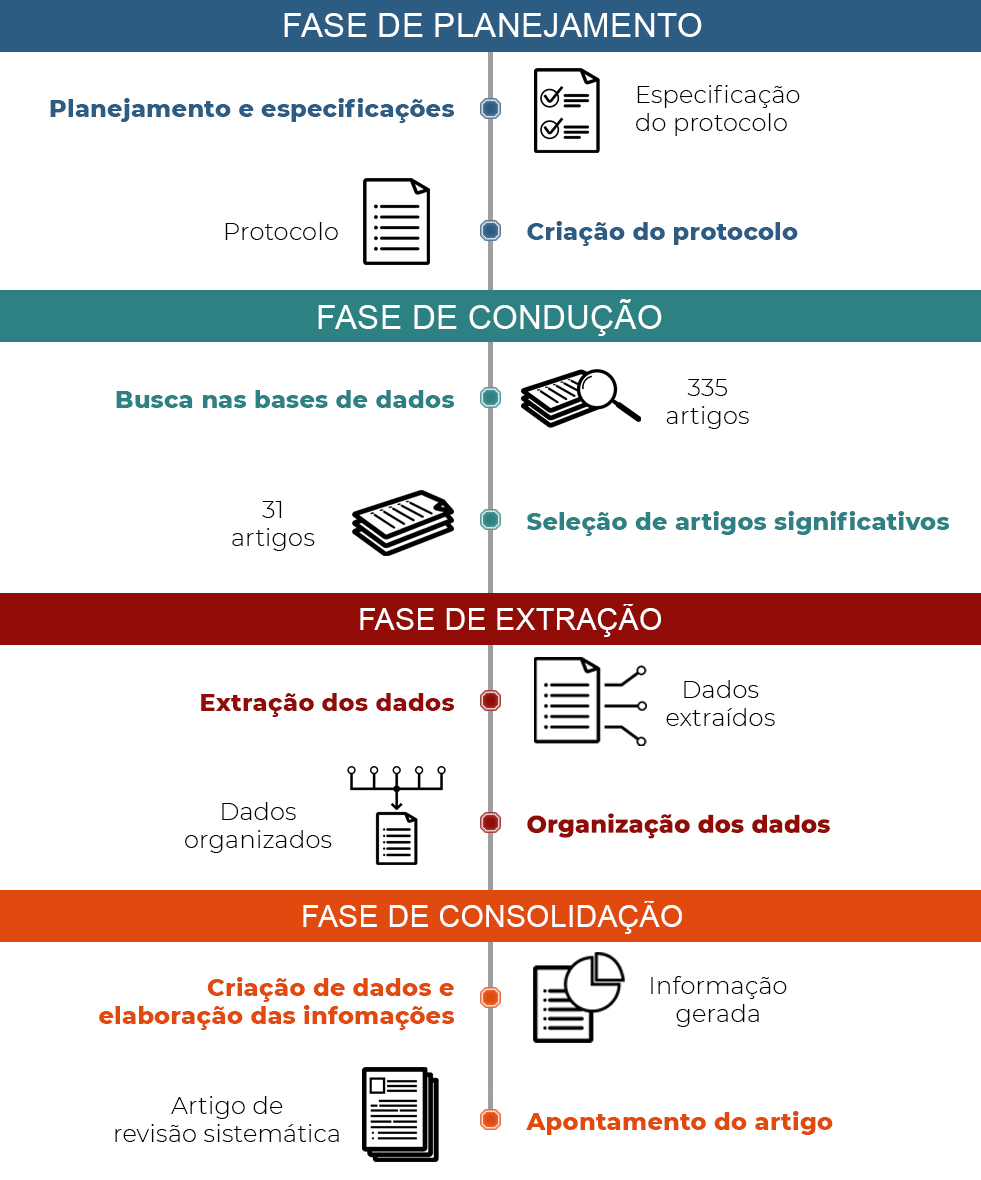
\includegraphics[scale=.40]{imagens/processo_revisao_sistematica.jpg}
    \label{fig:processo_revisao_sistematica}
    \source{Danilo Assunção, 2021}
\end{figure}

Na etapa de planejamento foi levantada junto ao protocolo a distinta questão:
``Quais são os métodos que sejam o estado da arte, para identificação de espécies utilizando Redes Neurais Convolucionais por meio de imagens digitais?''.
A conclusão desta pergunta veio a partir de bases de dados junto às seguintes strings de busca:

\begin{itemize}
  \item \textbf{IEEE Xplore} - (``convolutional neural network'' OR ``cnn'' OR ``convolution'') AND ``feature extraction'' AND (``insect'' OR ``pest'') AND (``image'' OR ``image segmentation'' OR ``image recognition'')
  \item \textbf{SCOPUS} - (``convolutional neural network'' OR ``cnn'' OR ``convolution'') AND ``feature extraction'' AND (``insect'' OR ``pest'') AND (``image'' OR ``image segmentation'' OR ``image recognition'') AND (EXCLUDE (DOCTYPE, ``cp'') OR EXCLUDE (DOCTYPE, ``re'') OR EXCLUDE (DOCTYPE, ``bk'') OR EXCLUDE (DOCTYPE, ``ch''))
\end{itemize}

Este trabalho foi conduzido de dezembro de 2020 até fevereiro de 2021. Inicialmente 335 trabalhos foram encontrados nas bases de dados especificadas acima, dos quais 302 estavam na base de dados SCOPUS e 33 na base de dados IEEE Xplore.

Após aplicar os critérios de inclusão e exclusão nos trabalhos coletados, 31 artigos foram selecionados e analisados por completo, sendo 28 da base SCOPUS e 3 da base IEEE Xplore.

Os critérios utilizados para incluir ou excluir um trabalho nesta revisão foram:

\begin{itemize}
  \item Inclusão
    \begin{itemize}
        \item{Artigos que utilizam Redes Neurais Convolucionais como ferramenta para discriminação de espécies por meio de imagens digitais;}
        \item{Artigos que contém técnicas computacionais de segmentação e extração de características de imagens digitais de diversas espécies biológicas;}
        \item{Artigos devem ter data de publicação maior ou igual a 2015.}
    \end{itemize}
  \item Exclusão
    \begin{itemize}
        \item{Artigos que não são relacionados com conceitos envolvendo técnicas de segmentação e extração de características por meio de imagens digitais;}
        \item{Artigos que não utilizam Redes Neurais Convolucionais para classificação automática de espécies por meio de imagens digitais;}
        \item{Artigos que não foram escritos com o idioma inglês ou português;}
        \item{Artigos com data de publicação menor que 2015;}
        \item{Documentos que não estejam categorizados como artigo em seu tipo de documento.}
    \end{itemize}
\end{itemize}

De cada trabalho selecionado foram extraídos os seguintes atributos: Ano de publicação, País de afiliação dos pesquisadores, Técnicas de pré-processamento de imagens, Arquitetura das Redes Neurais Convolucionais, Métodos de classificação, Técnica de aprendizado por transferência, Técnicas de aumento de dados.

Com a finalidade de poder encontrar possíveis lapsos nas pesquisas utilizadas, seguidamente da extração de dados, foi exercida uma averiguação sobre os principais obstáculos e propensões praticadas.

\section{Resultado da revisão sistemática}

Os 31 trabalhos selecionados foram estudados e os seguintes atributos foram extraídos: técnica de extração de características, tipos de características extraídas, principal país de afiliação dos pesquisadores e ano de publicação. Um breve sumário dos trabalhos com os respectivos dados extraídos encontram-se no Tabela \ref{tab:sumario_artigos_selecionados}.

% -----------------------------------------
% TABELA - SUMÁRIO DOS ARTIGOS ANALISADOS
% -----------------------------------------
%\begin{table}[h]
%\centering
%\caption{Sumário de todos os artigos analisados}
%\label{tab:sumario_artigos_selecionados}
%\resizebox{\textwidth}{!}{%
%\footnotesize
%\begin{tabular}{|p{1.5cm}|p{1.15cm}|p{1.2cm}|p{1.3cm}|p{1.3cm}|p{2.5cm}|p{2.5cm}|p{1.5cm}|}

\begin{landscape}
\begin{OnehalfSpacing}
\begin{footnotesize}
\begin{longtable}{|p{2.3cm}|p{1.3cm}|p{2cm}|p{2.6cm}|p{2.4cm}|p{4.3cm}|p{4.3cm}|p{2.5cm}|}
\caption{Sumário de todos os artigos analisados} \label{tab:sumario_artigos_selecionados} \\

\hline \textbf{Artigo} &
  \textbf{Ano de publicação} &
  \textbf{País de afiliação dos autores} &
  \textbf{Téc. de pré- processamento de imagens} &
  \textbf{Téc. de aprendizado por transferência} &
  \textbf{Téc. de aumento de dados} &
  \textbf{Modelo de arquitetura da CNN} &
  \textbf{Modelo do classificador} \\ \hline
\endfirsthead

\multicolumn{8}{c}%
{{\bfseries \tablename\ \thetable{} -- continuação da página anterior}} \\
\hline \textbf{Artigo} &
  \textbf{Ano de publicação} &
  \textbf{País de afiliação dos autores} &
  \textbf{Téc. de pré- processamento de imagens} &
  \textbf{Téc. de aprendizado por transferência} &
  \textbf{Téc. de aumento de dados} &
  \textbf{Modelo de arquitetura da CNN} &
  \textbf{Modelo do classificador} \\ \hline
\endhead

\hline \multicolumn{8}{|r|}{{Continua na próxima página}} \\ \hline
\endfoot

\hline \multicolumn{8}{|c|}{Fonte: Danilo Assunção, 2021} \\ \hline
\endlastfoot

\cite{liu2020classification} &
  2020 &
  Estados Unidos &
  Não aplicado &
  Fine-tuning &
  Skewing, Elastic distortion, Rotation &
  LeNet-5, AlexNet, VGGNet-16, VGGNet-19, ResNet-50, Inception v3, InceptionResNet v2 &
  Camada totalmente conectada \\ \hline
\cite{le2020automated} &
  2020 &
  França & 
  Resize &
  Fine-tuning &
  Constant to each channel, Split the channels of image &
  EB-Net &
  Camada totalmente conectada \\ \hline
\cite{zhangautomatic} &
  2020 &
  China &
  Não especificado &
  Não especificado &
  Não especificado &
  DenseNet-121 &
  Não especificado \\ \hline
\cite{liu2020grape} &
  2020 &
  China &
  Não aplicado &
  Não aplicado &
  High brightness, Low brightness, High contrast, Low contrast, High sharpness, Low sharpness, Rotation, Vertical symmetry, Horizontal symmetry, Gaussian noise, PCA Jittering &
  DICNN &
  Camada totalmente conectada \\ \hline
\cite{lu2020identifying} &
  2020 &
  Taiwan &
  Resize &
  Fine-tuning &
  Horizontal flipping, Vertical flipping, Width shifting, Height shifting, Rotation, Shearing, Zooming &
  VGGNet-16 &
  Camada totalmente conectada \\ \hline
\cite{banan2020deep} &
  2020 &
  Irã &
  Resize &
  Fine-tuning &
  Rotation, Height shifting, Width shifting &
  VGGNet-16 &
  Camada totalmente conectada \\ \hline
\cite{tiwari2020comparative} &
  2020 &
  India &
  Não especificado &
  Não aplicado &
  Não aplicado &
  CNN &
  Camada totalmente conectada \\ \hline
\cite{li2020using} &
  2020 &
  China &
  Cropping, Resize &
  Não aplicado &
  Rotation, Clipping &
  VGGNet-16, Inception v3 &
  Camada totalmente conectada \\ \hline
\cite{chen2020research} &
  2020 &
  China &
  Resize &
  Fine-tuning &
  Rotation, Blurred, Occluded &
  ResNeXt-101 &
  Camada totalmente conectada \\ \hline
\cite{hongclassification} &
  2020 &
  China &
  Resize, Cropping &
  Fine-tuning &
  Gaussian filter, Contrast enhancement &
  AlexNet &
  Camada totalmente conectada \\ \hline
\cite{rauf2019visual} &
  2019 &
  Paquistão, Estados Unidos &
  Resize, Transparent background &
  Não aplicado &
  Não aplicado &
  32-Layer CNN &
  Camada totalmente conectada \\ \hline
\cite{gomez2019coral} &
  2019 &
  Espanha, Dinamarca &
  Não especificado &
  Fine-tuning &
  Não especificado &
  Inception v3, ResNet-50, ResNet-152, DenseNet-121, DenseNet-161 &
  Camada totalmente conectada \\ \hline
\cite{cibuk2019efficient} &
  2019 &
  Turquia, Estados Unidos &
  Não aplicado &
  Feature transfer &
  Não aplicado &
  VGGNet-16, AlexNet &
  SVM (Kernel RBF) \\ \hline
\cite{li2019effective} &
  2019 &
  China &
  Resize &
  Não aplicado &
  Multi-scale, Rotation &
  ResNet-50 &
  Camada totalmente conectada \\ \hline
\cite{khalifa2019deep} &
  2019 &
  Egito, Luxemburgo &
  Não especificado &
  Não aplicado &
  Reflection, Zooming, Gaussian noise, Poisson noise, Salt and pepper noise, Speckle noise &
  CNN &
  Camada totalmente conectada \\ \hline
\cite{hsiang2019endless} &
  2019 &
  Suécia, Reino Unido &
  Resize &
  Fine-tuning &
  Não especificado &
  VGGNet-16, DenseNet-121, Inception v3 &
  Camada totalmente conectada \\ \hline
\cite{ren2019feature} &
  2019 &
  Japão &
  Resize, Cropping &
  Não aplicado &
  Resize, Cropping, Mean and standard deviation normalization &
  FR-ResNet &
  Camada totalmente conectada \\ \hline
\cite{valan2019automated} &
  2019 &
  Suécia &
  Resize, Cropping &
  Feature transfer &
  Não aplicado &
  VGGNet-16 &
  SVM (Kernel Linear) \\ \hline
\cite{gyires2019deep} &
  2019 &
  Hungria &
  Cropping, Resize &
  Fine-tuning &
  Não aplicado &
  AlexNet, Inception V3 &
  Camada totalmente conectada \\ \hline
\cite{thenmozhi2019crop} &
  2019 &
  India &
  Gray scale, Canny Edge Detection, Cropping, Resize &
  Fine-tuning &
  Reflection, Scaling, Rotation, Translation &
  VGGNet-16, VGGNet-19 &
  Camada totalmente conectada \\ \hline
\cite{tetila2019deep} &
  2019 &
  Brasil &
  Não especificado &
  Fine-tuning, Feature transfer &
  Rotation, Scaling, Scrolling, Zooming &
  DenseNet-201, InceptionResNet v2, ResNet-50 &
  Camada totalmente conectada \\ \hline
\cite{wei2018deep} &
  2018 &
  Malasia &
  Resize, Padding &
  Não aplicado &
  Não aplicado &
  D-Leaf &
  Camada totalmente conectada \\ \hline
\cite{zhu2018method} &
  2018 &
  China &
  Não especificado &
  Não aplicado &
  Não aplicado &
  Inception v2 &
  Camada totalmente conectada \\ \hline
\cite{zhu2018plant} &
  2018 &
  China &
  Resize &
  Não especificado &
  Não aplicado &
  CNN &
  SVM (Kernel Linear) \\ \hline
\cite{villon2018deep} &
  2018 &
  França &
  Não especificado &
  Não aplicado &
  Não aplicado &
  GoogLeNet &
  Camada totalmente conectada \\ \hline
\cite{lee2017deep} &
  2017 &
  Malásia, Reino Unido &
  Resize &
  Fine-tuning &
  Rotation &
  CNN &
  Camada totalmente conectada \\ \hline
\cite{zielinski2017deep} &
  2017 &
  Polônia &
  Não especificado &
  Feature transfer &
  Não aplicado &
  AlexNet, VGGNet-M, VGGNet-VD &
  SVM (Kernel Linear, RBF e Polinomial), Random Forest \\ \hline
\cite{wang2017crop} &
  2017 &
  China &
  Não especificado &
  Não especificado &
  Não aplicado &
  LeNet-5, AlexNet &
  Camada totalmente conectada \\ \hline
\cite{lim2017performance} &
  2017 &
  Coreia do Sul &
  Resize, Cropping &
  Não especificado &
  Rotation, Zooming &
  AlexNet &
  Camada totalmente conectada \\ \hline
\cite{sun2017deep} &
  2017 &
  China &
  Não especificado &
  Não aplicado &
  Não aplicado &
  ResNet-26 &
  Camada totalmente conectada \\ \hline
  
\end{longtable}
\end{footnotesize}
\end{OnehalfSpacing}
\end{landscape}

\subsection{Ano de publicação}

Nesta revisão sistemática foi coletado o ano de publicação dos artigos para ser feito uma analise de tendencia referente aos assuntos que abordam técnicas de reconhecimento de espécies utilizando Redes Neurais Convolucionais. Na Figura \ref{fig:grafico_ano_vs_publicacao} é fornecida a quantidade de artigos selecionados com base em seu ano de publicação.

\begin{figure}[H]
    \centering
    \caption{Ano de publicação dos artigos selecionados}
    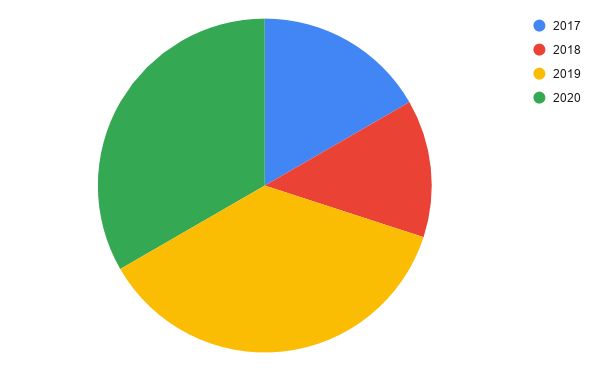
\includegraphics[scale=.60]{imagens/grafico_ano_vs_publicacao.png}
    \label{fig:grafico_ano_vs_publicacao}
    \source{Danilo Assunção, 2021}
\end{figure}

Nota-se que a maior quantidade dos artigos selecionados foram publicados em 2019, representando um total de 36,67\% (11). Já em 2020, é tido 33,33\% (10) dos artigos. Em 2018 a quantia de artigos foi de 13,33\% (4) e em 2017, 16,67\% (5).

É possível perceber que, de 2017 até 2019 houve um aumento significativo da aplicação de Redes Neurais Convolucionais para a resolução de problemas envolvendo reconhecimento automático de imagens. Entretanto, de 2019 para 2020 houve uma leve queda em consideração aos artigos abordados, mas isto não necessariamente prova que a tendência ao assunto abordado diminuiu. 

Afim de metrificar e visando uma melhor compreensão sobre a quantidade de publicações com base em assuntos que envolvem reconhecimento automático de espécies utilizando técnicas de aprendizado profundo, foi elaborado um gráfico com todos os artigos encontrados na base de dados pela consulta feita nas bases do SCOPUS e IEEE Xplore. Na Figura \ref{fig:grafico_ano_vs_quantidade} é mostrando uma linha de tendência com relação aos assuntos envolvendo as palavras chaves a respeito de aprendizado profundo e Redes Neurais Convolucionais.

\begin{figure}[H]
    \centering
    \caption{Ano de publicação dos artigos com base em palavras chave}
    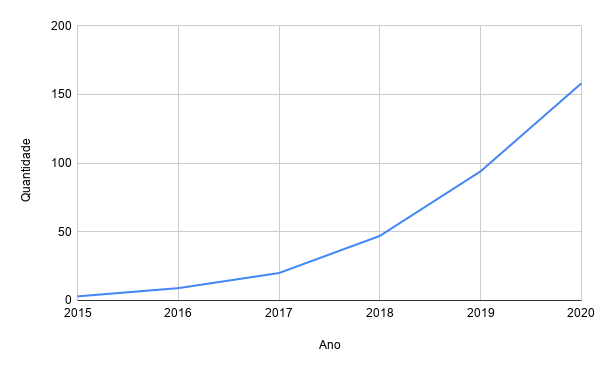
\includegraphics[scale=.60]{imagens/grafico_ano_vs_quantidade.png}
    \label{fig:grafico_ano_vs_quantidade}
    \source{Danilo Assunção, 2021}
\end{figure}

\subsection{País de afiliação dos autores}

Foi feito a extração de dados sobre os países de cada pesquisador contribuinte em determinado artigo e esta visão pode ser na partir da Figura \ref{fig:grafico_pais_vs_publicacao}.

\begin{figure}[H]
    \centering
    \caption{País de afiliação dos pesquisadores}
    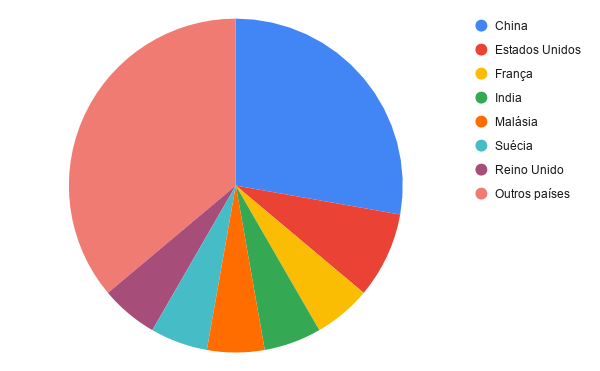
\includegraphics[scale=.60]{imagens/grafico_pais_vs_publicacao.png}
    \label{fig:grafico_pais_vs_publicacao}
    \source{Danilo Assunção, 2021}
\end{figure}

Pode ser visto que, com base nos artigos selecionados, a China possui a liderança com relação à produção de artigos científicos relacionados a identificação e classificação de espécies por meio do uso de Redes Neurais Convolucionais, possuindo 27,78\% (10 artigos) em relação aos pesquisadores de outros países. Os Estados Unidos, em segundo colocado, possuindo 8,33\% (3 artigos). A França, Índia, Malásia, Suécia e o Reino Unido possuem ambos 5,56\% (2 artigos) artigos publicados. Já na categoria ``Outros países'', que compõe os 36,11\% dos artigos publicados restantes, são as demais regiões que possuem em cada um deles somente apenas um artigo cientifico publicado.

\subsection{Técnicas de pré-processamento de imagens}

Nos métodos abordados nos artigos selecionados é possível identificar a utilização de técnicas de pré-processamento de imagens em alguns cenários distintos como é demonstrado na Figura \ref{fig:grafico_preprocessamento_vs_uso}.

\begin{figure}[H]
    \centering
    \caption{Técnicas de pré-processamento de imagens aplicadas}
    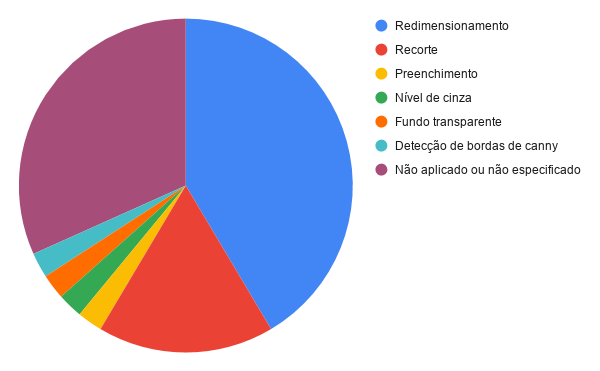
\includegraphics[scale=.60]{imagens/grafico_preprocessamento_vs_uso.png}
    \label{fig:grafico_preprocessamento_vs_uso}
    \source{Danilo Assunção, 2021}
\end{figure}

O desempenho da tarefa de classificação é melhorado ao aplicar as técnicas de pré-processamento de imagem para extrair automaticamente o resultado da imagem introduzida antes de ser inserida nos modelos de aprendizagem profunda \cite{thenmozhi2019crop}. A técnica de Redimensionamento (\textit{resize}) vem liderando com 41,46\% de uso com relação as outras estratégias abordadas, e isso se deve aos diversos fatores que auxiliam no aumento de performance das redes neurais convolucionais, como a quantidade reduzida de parâmetros a serem introduzidos na rede. Em segundo com 17,07\%, o Recorte (\textit{cropping}) que pode vir a ser utilizado para destacar a região de interesse da imagem e reduzindo também o tamanho da imagem \cite{thenmozhi2019crop}. Preenchimento (\textit{padding}), Nível de cinza (\textit{gray scale}), Fundo transparente (\textit{transparent background}) e Detecção de bordas de canny (\textit{canny edge detection}) foram algumas das abordagens utilizadas, e ocupam apenas 2,44\% de uso com relação aos outros métodos. Ocupando os 31,71\% restantes, foram artigos que não aplicaram ou não especificaram diretamente o uso de técnicas de pré-processamento de imagens, isto pode ser ocasionado pelo fato do conjunto de dados utilizado já estar previamente pré-processado em sua disponibilização, ou de não haver necessidade direta de uma preparação antes de introduzi-las à rede.

\subsection{Técnica de aprendizado por transferência}

Aprendizado por transferência (\textit{Transfer learning}) é uma técnica que permite a utilização de uma rede pré-treinada, reduzindo a carga computacional e beneficiando-se do poder de uma Rede Neural Convolucional mais sofisticada \cite{valan2019automated}. Na Figura \ref{fig:grafico_transfer-learning_vs_uso} será apresentado os dados coletados por meios dos artigos analisados.

\begin{figure}[H]
    \centering
    \caption{Técnicas de Aprendizado por transferência}
    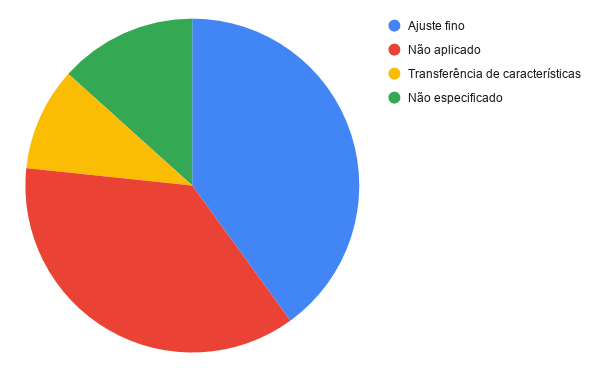
\includegraphics[scale=.60]{imagens/grafico_transfer-learning_vs_uso.png}
    \label{fig:grafico_transfer-learning_vs_uso}
    \source{Danilo Assunção, 2021}
\end{figure}

O ajuste fino (\textit{Fine-tuning}) foi o método mais utilizado com 40,00\% (12) de uso em relação a todas as outras técnicas encontradas nos artigos analisados. Podendo ser devido ao Ajuste fino que tende a funcionar bem quando a tarefa especializada é semelhante à tarefa original \cite{valan2019automated}, e este mecanismo foi utilizado para diversas tarefas com cenários semelhantes de reconhecimento de padrões. Em segundo, é tido em todos os artigos que não aplicaram nenhuma técnica de Aprendizado por transferência ocupando 36,67\% (11), devendo-se ao fato de que nem todo cenário pode vir a necessitar do uso de técnica de reaproveitamento deste tipo, e também, este mecanismo é suscetível a sobreajuste na tarefa especializada quando os conjuntos de dados são pequenos, pois pode associar incorretamente uma categoria rara a um recurso irrelevante, como um tipo especial de fundo, que por acaso está presente nas poucas imagens dessa categoria e no conjunto de treinamento \cite{valan2019automated}. Transferência de características (\textit{Feature transfer}) envolve o uso da Rede Neural Convolucional pré-treinada como um extrator de características automatizado \cite{valan2019automated}, este método teve um uso de 10,00\% (3) com relação às outras técnicas abordadas. O restante mapeado, com 13,33\% (4) não especificou diretamente o tipo de mecanismo de Aprendizado por transferência utilizado.

\subsection{Técnicas de aumento de dados}

Métodos de Aumento de dados (\textit{Data augmentation}) permite aumentar artificialmente o tamanho do conjunto de treinamento. O aumento do conjunto de treinamento é feito ao aplicar várias distorções às imagens originais, como zoom, virando-as horizontalmente ou verticalmente, girando-as, deslocando-as e dentre outros \cite{gomez2019coral}. Na Figura \ref{fig:grafico_aumento-dados_vs_uso} é demonstrado graficamente as técnicas utilizadas para o Aumento de dados nos artigos abordados.

\begin{figure}[H]
    \centering
    \caption{Técnicas de Aumento de dados}
    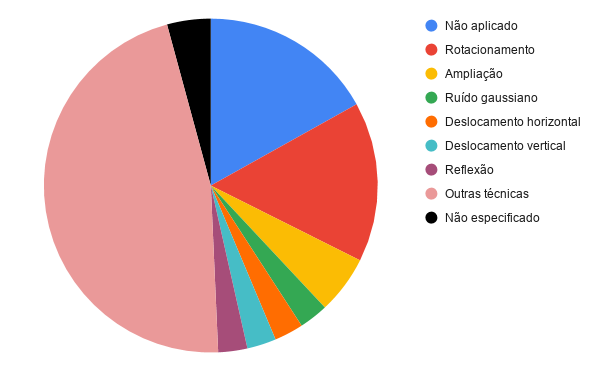
\includegraphics[scale=.60]{imagens/grafico_aumento-dados_vs_uso.png}
    \label{fig:grafico_aumento-dados_vs_uso}
    \source{Danilo Assunção, 2021}
\end{figure}

Em maioria, os artigos não aplicaram técnicas de Aumento de dados, com uma representação de 16,90\% (12) de todos os exemplares analisados, isto pode ser ocasionado pelo fato dos conjuntos de dados utilizados pelos autores já forem grandes o suficiente ou devido ao uso de outras técnicas para supressão de sobreajuste. Em seguida, é possível observar que as técnicas de Aumento de dados utilizando Rotacionamento (\textit{Rotation}) são bem prioritárias quando este mecanismo é aplicado, com um total de uso de 15,49\% (11) com relação aos outros meios. Ampliação (\textit{Zooming}), sendo a terceira metodologia mais aplicada com 5,63\% (4). Ruído gaussiano (\textit{Gaussian noise}), Deslocamento horizontal (\textit{Width shifting}), Deslocamento vertical (\textit{Height shifting}) e Reflexão (\textit{Reflection}) representando 2,82\% (2) nos demais cenários. As Outras técnicas agrupadas são métodos que foram utilizados somente uma única vez e o conjunto não especificado são aos artigos que não esclareceram de maneira explicita o tipo de técnica de Aumento de dados utilizada.

\subsection{Modelo de arquitetura da CNN}

É possível identificar na literatura uma grande quantidade de arquiteturas de Redes Neurais Convolucionais sendo utilizadas em diversas soluções de problemas que envolvem a classificação morfológica de espécies, por meio de suas imagens digitais. Na Figura \ref{fig:grafico_arquitetura_vs_uso} é possível observar graficamente estes dados.

\begin{figure}[H]
    \centering
    \caption{Arquitetura de Redes Neurais Convolucionais}
    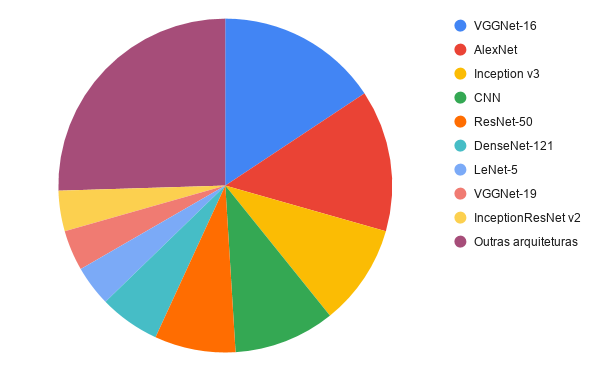
\includegraphics[scale=.60]{imagens/grafico_arquitetura_vs_uso.png}
    \label{fig:grafico_arquitetura_vs_uso}
    \source{Danilo Assunção, 2021}
\end{figure}

A VGGNet-16 obteve uma utilização de 14,29\% (8), encontrando-se em primeiro com relação as outras arquiteturas destacadas. Em comparação a AlexNet posicionada em segundo com 12,50\% (7), as arquiteturas de VGGNet aumentam a profundidade da rede e reduz o tamanho do \textit{kernel} de convolução, podendo assim reduzir os parâmetros a serem computados, além disso, o desempenho de generalização de arquiteturas VGGNet costumam ter bons resultados \cite{li2020using}. Os modelos de Inception v3 e CNN, onde a categoria CNN representa os modelos implementados pelos autores em seus artigos ocupam 7,81\% (5). ResNet-50 com 6,25\% (4) e DenseNet-121 com 4,69\% (3). LeNet-5, VGGNet-19 e InceptionResNet v2 que ocupam 3,13\% (2) em aplicabilidade. Já as ``Outras arquiteturas'' que compõe 20,31\% do restante das arquiteturas utilizadas, possuem uma única utilização em seus respectivos artigos.

Para uma diferente perspectiva de visualização de usabilidade das arquiteturas de Redes Neurais Convolucionais extraídas nos projetos em questão, foi feito um agrupamento por tipo de arquitetura para a identificação dos exemplares mais utilizados, como é demonstrado na Figura \ref{fig:grafico_arquitetura_agrupada_vs_uso}.

\begin{figure}[H]
    \centering
    \caption{Tipos agrupados de arquiteturas de Redes Neurais Convolucionais}
    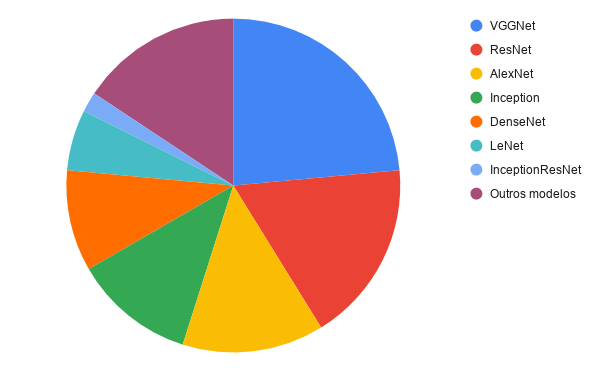
\includegraphics[scale=.60]{imagens/grafico_arquitetura_agrupada_vs_uso.png}
    \label{fig:grafico_arquitetura_agrupada_vs_uso}
    \source{Danilo Assunção, 2021}
\end{figure}

Nota-se que modelos de VGGNet com uso de 23,53\% (12) ainda dominam em termos de arquiteturas aplicadas na resolução de problemas envolvendo a identificação de espécies. Arquiteturas do tipo ResNet ocupam o segundo lugar com 17,65\% (9), isso devido ao seu comportamento de aumentar a profundidade da rede, sendo assim, as ResNets oferecem melhores recursos de aproximação de função (convergência ao resultado) à medida em que ganham mais parâmetros, contribuindo com sucesso na resolução de problemas como os de dissipação de gradiente, onde alguns modelos mais tradicionais acabam não conseguindo soluciona-lo, tendo resultados inferiores ao desejado \cite{sun2017deep}. Tendo a AlexNet em terceiro com 13,73\% (7), sendo este tipo de arquitetura um modelo pré-treinado de rede neural convolucional que permite a aplicação de Aprendizado por Transferência para que atinja melhores resultados \cite{hongclassification}. Modelos de Inception 11,76\% (6), DenseNet 9,80\% (5). LeNet 5,88\% (5) e InceptionResNet 1,96\% (1) possuem a menor quantidade de uso para os cenários avaliados. Por último, os ``Outros modelos'' que são arquiteturas de CNN desenvolvidas pelos autores dos artigos com especificidade para solucionar seus respectivos problemas abordados.

\subsection{Modelo do classificador}

Os métodos de classificação são aplicados nas últimas camadas das Redes Neurais Convolucionais, utilizando as características extraídas como entrada para o processo de classificação dos dados e predição do resultado. Na Figura \ref{fig:grafico_classificador_vs_uso} é demonstrado os exemplares aplicados nos artigos selecionados.

\begin{figure}[H]
    \centering
    \caption{Método de classificação utilizado}
    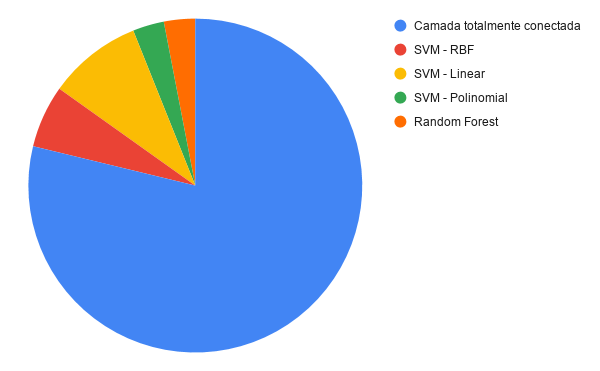
\includegraphics[scale=.60]{imagens/grafico_classificador_vs_uso.png}
    \label{fig:grafico_classificador_vs_uso}
    \source{Danilo Assunção, 2021}
\end{figure}


A partir do processo de convolução da Rede Neural Convolucional, é seguido o agrupamento e divisão das imagens em recursos. Em sequência desse processo, tais recursos são utilizados para alimentar a estrutura de rede neural totalmente conectada, pode direcionar a decisão de classificação final \cite{rauf2019visual}. 

Decorrendo em 78,79\% (26) de utilização apresentada nos artigos e representada como ``Camada totalmente conectada''. Nos demais cenários onde a rede neural convolucional é utilizada somente para extração de características, é visto a aplicação conjunta com algoritmos de SVM (Máquina de vetores de suporte) com \textit{kernel} Linear 9,09\% (3), RBF (Função de Base Radial) 6,06\% (2) e Polinomial 3,03\% (1). Por fim, houve apenas uma implementação do algoritmo \textit{Random Forest} ocupando 3,03\% (1).

\section{Conclusão}

Após o término da revisão sistemática é perceptível que o uso de técnicas de aprendizado profundo, como redes neurais convolucionais, vem sendo empregadas em diversos cenários onde há a necessidade de otimização no processo de extração de características das imagens, para assim, solucionar problemas que envolvem reconhecimento de espécies. Um dos atributos mais importantes é a sua capacidade de aprender as características de mais alto nível de uma imagem, e fornecer prontamente uma quantidade de informações relevantes que permitam que os algoritmos de classificação possam identificar com mais eficácia o objeto visualizado. Entretanto, é importante ressaltar que o uso deste mecanismo exige uma quantidade muito grande de dados, justamente para que seu resultado venha a convergir para um modelo que tenha a capacidade de efetivar tal atividade, e para isto foi observado na literatura o uso de técnicas como transferência de aprendizado e aumento de dados que permitem a utilização de redes neurais convolucionais, mesmo com um conjunto pequeno de dados disponíveis e demonstrando também que o uso de pré-processamento ainda pode vir a ser extremamente útil em cenários diversos envolvendo processamento de imagens digitais.

\chapter{Mais uma outra seção primária}

Texto de exemplo, texto de exemplo, texto de exemplo, texto de exemplo, texto de exemplo, texto de exemplo, texto de exemplo, texto de exemplo, texto de exemplo, texto de exemplo, texto de exemplo, texto de exemplo, texto de exemplo, texto de exemplo, texto de exemplo, texto de exemplo, texto de exemplo, texto de exemplo, texto de exemplo, texto de exemplo, texto de exemplo, texto de exemplo, texto de exemplo.

Texto de exemplo, texto de exemplo, texto de exemplo, texto de exemplo, texto de exemplo, texto de exemplo, texto de exemplo, texto de exemplo, texto de exemplo, texto de exemplo, texto de exemplo, texto de exemplo, texto de exemplo, texto de exemplo, texto de exemplo, texto de exemplo, texto de exemplo, texto de exemplo, texto de exemplo, texto de exemplo, texto de exemplo, texto de exemplo.

\section{Uma seção secundária}

Texto de exemplo, texto de exemplo, texto de exemplo, texto de exemplo, texto de exemplo, texto de exemplo, texto de exemplo, texto de exemplo, texto de exemplo, texto de exemplo, texto de exemplo, texto de exemplo, texto de exemplo, texto de exemplo, texto de exemplo, texto de exemplo, texto de exemplo, texto de exemplo, texto de exemplo, texto de exemplo, texto de exemplo, texto de exemplo, texto de exemplo.

Texto de exemplo, texto de exemplo, texto de exemplo, texto de exemplo, texto de exemplo, texto de exemplo, texto de exemplo, texto de exemplo, texto de exemplo, texto de exemplo, texto de exemplo, texto de exemplo, texto de exemplo, texto de exemplo, texto de exemplo, texto de exemplo, texto de exemplo, texto de exemplo, texto de exemplo, texto de exemplo, texto de exemplo, texto de exemplo, texto de exemplo.

\subsection{Uma seção terciária}

Texto de exemplo, texto de exemplo, texto de exemplo, texto de exemplo, texto de exemplo, texto de exemplo, texto de exemplo, texto de exemplo, texto de exemplo, texto de exemplo, texto de exemplo, texto de exemplo, texto de exemplo, texto de exemplo, texto de exemplo, texto de exemplo, texto de exemplo, texto de exemplo, texto de exemplo, texto de exemplo, texto de exemplo, texto de exemplo, texto de exemplo.


\subsection{Outra seção terciária}

Texto de exemplo, texto de exemplo, texto de exemplo, texto de exemplo, texto de exemplo, texto de exemplo, texto de exemplo, texto de exemplo, texto de exemplo, texto de exemplo, texto de exemplo, texto de exemplo, texto de exemplo, texto de exemplo, texto de exemplo, texto de exemplo, texto de exemplo, texto de exemplo, texto de exemplo, texto de exemplo, texto de exemplo, texto de exemplo, texto de exemplo.

\subsection{Mais uma seção terciária}

Texto de exemplo, texto de exemplo, texto de exemplo, texto de exemplo, texto de exemplo, texto de exemplo, texto de exemplo, texto de exemplo, texto de exemplo, texto de exemplo, texto de exemplo, texto de exemplo, texto de exemplo, texto de exemplo, texto de exemplo, texto de exemplo, texto de exemplo, texto de exemplo, texto de exemplo, texto de exemplo, texto de exemplo, texto de exemplo, texto de exemplo.

Texto de exemplo, texto de exemplo, texto de exemplo, texto de exemplo, texto de exemplo, texto de exemplo, texto de exemplo, texto de exemplo, texto de exemplo, texto de exemplo, texto de exemplo, texto de exemplo, texto de exemplo, texto de exemplo, texto de exemplo, texto de exemplo, texto de exemplo, texto de exemplo, texto de exemplo, texto de exemplo, texto de exemplo, texto de exemplo, texto de exemplo.

\section{Outra seção secundária}

Texto de exemplo, texto de exemplo, texto de exemplo, texto de exemplo, texto de exemplo, texto de exemplo, texto de exemplo, texto de exemplo, texto de exemplo, texto de exemplo, texto de exemplo, texto de exemplo, texto de exemplo, texto de exemplo, texto de exemplo, texto de exemplo, texto de exemplo, texto de exemplo, texto de exemplo, texto de exemplo, texto de exemplo, texto de exemplo, texto de exemplo.

Texto de exemplo, texto de exemplo, texto de exemplo, texto de exemplo, texto de exemplo, texto de exemplo, texto de exemplo, texto de exemplo, texto de exemplo, texto de exemplo, texto de exemplo, texto de exemplo, texto de exemplo, texto de exemplo, texto de exemplo, texto de exemplo, texto de exemplo, texto de exemplo, texto de exemplo, texto de exemplo, texto de exemplo, texto de exemplo, texto de exemplo.

Texto de exemplo, texto de exemplo, texto de exemplo, texto de exemplo, texto de exemplo, texto de exemplo, texto de exemplo, texto de exemplo, texto de exemplo, texto de exemplo, texto de exemplo, texto de exemplo, texto de exemplo, texto de exemplo, texto de exemplo, texto de exemplo, texto de exemplo, texto de exemplo, texto de exemplo, texto de exemplo, texto de exemplo, texto de exemplo, texto de exemplo.

\section{Mais uma seção secundária}

Texto de exemplo, texto de exemplo, texto de exemplo, texto de exemplo, texto de exemplo, texto de exemplo, texto de exemplo, texto de exemplo, texto de exemplo, texto de exemplo, texto de exemplo, texto de exemplo, texto de exemplo, texto de exemplo, texto de exemplo, texto de exemplo, texto de exemplo, texto de exemplo, texto de exemplo, texto de exemplo, texto de exemplo, texto de exemplo, texto de exemplo.

Texto de exemplo, texto de exemplo, texto de exemplo, texto de exemplo, texto de exemplo, texto de exemplo, texto de exemplo, texto de exemplo, texto de exemplo, texto de exemplo, texto de exemplo, texto de exemplo, texto de exemplo, texto de exemplo, texto de exemplo, texto de exemplo, texto de exemplo, texto de exemplo, texto de exemplo, texto de exemplo, texto de exemplo, texto de exemplo, texto de exemplo.

\chapter{Conclusão}

Texto de exemplo, texto de exemplo, texto de exemplo, texto de exemplo, texto de exemplo, texto de exemplo, texto de exemplo, texto de exemplo, texto de exemplo, texto de exemplo, texto de exemplo, texto de exemplo, texto de exemplo, texto de exemplo, texto de exemplo, texto de exemplo, texto de exemplo, texto de exemplo, texto de exemplo, texto de exemplo, texto de exemplo, texto de exemplo, texto de exemplo.

Texto de exemplo, texto de exemplo, texto de exemplo, texto de exemplo, texto de exemplo, texto de exemplo, texto de exemplo, texto de exemplo, texto de exemplo, texto de exemplo, texto de exemplo, texto de exemplo, texto de exemplo, texto de exemplo, texto de exemplo, texto de exemplo, texto de exemplo, texto de exemplo, texto de exemplo, texto de exemplo, texto de exemplo, texto de exemplo.

\section{Uma seção secundária}

Texto de exemplo, texto de exemplo, texto de exemplo, texto de exemplo, texto de exemplo, texto de exemplo, texto de exemplo, texto de exemplo, texto de exemplo, texto de exemplo, texto de exemplo, texto de exemplo, texto de exemplo, texto de exemplo, texto de exemplo, texto de exemplo, texto de exemplo, texto de exemplo, texto de exemplo, texto de exemplo, texto de exemplo, texto de exemplo, texto de exemplo.

Texto de exemplo, texto de exemplo, texto de exemplo, texto de exemplo, texto de exemplo, texto de exemplo, texto de exemplo, texto de exemplo, texto de exemplo, texto de exemplo, texto de exemplo, texto de exemplo, texto de exemplo, texto de exemplo, texto de exemplo, texto de exemplo, texto de exemplo, texto de exemplo, texto de exemplo, texto de exemplo, texto de exemplo, texto de exemplo, texto de exemplo.

\subsection{Uma seção terciária}

Texto de exemplo, texto de exemplo, texto de exemplo, texto de exemplo, texto de exemplo, texto de exemplo, texto de exemplo, texto de exemplo, texto de exemplo, texto de exemplo, texto de exemplo, texto de exemplo, texto de exemplo, texto de exemplo, texto de exemplo, texto de exemplo, texto de exemplo, texto de exemplo, texto de exemplo, texto de exemplo, texto de exemplo, texto de exemplo, texto de exemplo.

\subsection{Outra seção terciária}

Texto de exemplo, texto de exemplo, texto de exemplo, texto de exemplo, texto de exemplo, texto de exemplo, texto de exemplo, texto de exemplo, texto de exemplo, texto de exemplo, texto de exemplo, texto de exemplo, texto de exemplo, texto de exemplo, texto de exemplo, texto de exemplo, texto de exemplo, texto de exemplo, texto de exemplo, texto de exemplo, texto de exemplo, texto de exemplo, texto de exemplo.

\subsection{Mais uma seção terciária}

Texto de exemplo, texto de exemplo, texto de exemplo, texto de exemplo, texto de exemplo, texto de exemplo, texto de exemplo, texto de exemplo, texto de exemplo, texto de exemplo, texto de exemplo, texto de exemplo, texto de exemplo, texto de exemplo, texto de exemplo, texto de exemplo, texto de exemplo, texto de exemplo, texto de exemplo, texto de exemplo, texto de exemplo, texto de exemplo, texto de exemplo.

Texto de exemplo, texto de exemplo, texto de exemplo, texto de exemplo, texto de exemplo, texto de exemplo, texto de exemplo, texto de exemplo, texto de exemplo, texto de exemplo, texto de exemplo, texto de exemplo, texto de exemplo, texto de exemplo, texto de exemplo, texto de exemplo, texto de exemplo, texto de exemplo, texto de exemplo, texto de exemplo, texto de exemplo, texto de exemplo, texto de exemplo.

\section{Outra seção secundária}

Texto de exemplo, texto de exemplo, texto de exemplo, texto de exemplo, texto de exemplo, texto de exemplo, texto de exemplo, texto de exemplo, texto de exemplo, texto de exemplo, texto de exemplo, texto de exemplo, texto de exemplo, texto de exemplo, texto de exemplo, texto de exemplo, texto de exemplo, texto de exemplo, texto de exemplo, texto de exemplo, texto de exemplo, texto de exemplo, texto de exemplo.

Texto de exemplo, texto de exemplo, texto de exemplo, texto de exemplo, texto de exemplo, texto de exemplo, texto de exemplo, texto de exemplo, texto de exemplo, texto de exemplo, texto de exemplo, texto de exemplo, texto de exemplo, texto de exemplo, texto de exemplo, texto de exemplo, texto de exemplo, texto de exemplo, texto de exemplo, texto de exemplo, texto de exemplo, texto de exemplo, texto de exemplo.

Texto de exemplo, texto de exemplo, texto de exemplo, texto de exemplo, texto de exemplo, texto de exemplo, texto de exemplo, texto de exemplo, texto de exemplo, texto de exemplo, texto de exemplo, texto de exemplo, texto de exemplo, texto de exemplo, texto de exemplo, texto de exemplo, texto de exemplo, texto de exemplo, texto de exemplo, texto de exemplo, texto de exemplo, texto de exemplo, texto de exemplo.

\section{Mais uma seção secundária}

Texto de exemplo, texto de exemplo, texto de exemplo, texto de exemplo, texto de exemplo, texto de exemplo, texto de exemplo, texto de exemplo, texto de exemplo, texto de exemplo, texto de exemplo, texto de exemplo, texto de exemplo, texto de exemplo, texto de exemplo, texto de exemplo, texto de exemplo, texto de exemplo, texto de exemplo, texto de exemplo, texto de exemplo, texto de exemplo, texto de exemplo.

Texto de exemplo, texto de exemplo, texto de exemplo, texto de exemplo, texto de exemplo, texto de exemplo, texto de exemplo, texto de exemplo, texto de exemplo, texto de exemplo, texto de exemplo, texto de exemplo, texto de exemplo, texto de exemplo, texto de exemplo, texto de exemplo, texto de exemplo, texto de exemplo, texto de exemplo, texto de exemplo, texto de exemplo, texto de exemplo, texto de exemplo.

% ----------------------------------------------------------
% ELEMENTOS PÓS-TEXTUAIS
% ----------------------------------------------------------
\postextual
% ----------------------------------------------------------

% ----------------------------------------------------------
% Referências bibliográficas
% ----------------------------------------------------------
\bibliography{referencias}

% ----------------------------------------------------------
% Glossário
% ----------------------------------------------------------
%
% Consulte o manual da classe abntex2 para orientações sobre o glossário.
%
%\glossary

% ----------------------------------------------------------
% Apêndices
% ----------------------------------------------------------

% ---
% Inicia os apêndices
% ---
\begin{apendicesenv}

% Imprime uma página indicando o início dos apêndices
%\partapendices

%-------------------------------------------------------------------------
% Comentário adicional do PPgSI - Informações sobre ``apêndice''
%
% Para todos os captions/(títulos) (de seções, subseções, tabelas, 
% ilustrações, etc.):
%     - em maiúscula apenas a primeira letra da sentença (do título), 
%       exceto nomes próprios, geográficos, institucionais ou Programas ou
%       Projetos ou siglas, os quais podem ter letras em maiúscula também.
%
% Todas  as tabelas, ilustrações (figuras, quadros, gráficos etc. ), 
% anexos, apêndices devem obrigatoriamente ser citados no texto.
%      - a citação deve vir sempre antes da primeira vez em que a tabela, 
%        ilustração etc., aparecer pela primeira vez.
%
%-------------------------------------------------------------------------
\chapter{Exemplo de apêndice}

Texto de exemplo, texto de exemplo, texto de exemplo, texto de exemplo, texto de exemplo, texto de exemplo, texto de exemplo, texto de exemplo, texto de exemplo, texto de exemplo, texto de exemplo, texto de exemplo, texto de exemplo, texto de exemplo, texto de exemplo, texto de exemplo, texto de exemplo, texto de exemplo, texto de exemplo.

\section*{1 Exemplo de seção de apêndice não apresentada no sumário}

Texto de exemplo, texto de exemplo, texto de exemplo, texto de exemplo, texto de exemplo, texto de exemplo, texto de exemplo, texto de exemplo, texto de exemplo, texto de exemplo, texto de exemplo, texto de exemplo, texto de exemplo, texto de exemplo, texto de exemplo, texto de exemplo, texto de exemplo, texto de exemplo, texto de exemplo.

\subsection*{1.1 Exemplo de subseção de apêndice não apresentada no sumário}

Texto de exemplo, texto de exemplo, texto de exemplo, texto de exemplo, texto de exemplo, texto de exemplo, texto de exemplo, texto de exemplo, texto de exemplo, texto de exemplo, texto de exemplo, texto de exemplo, texto de exemplo, texto de exemplo, texto de exemplo, texto de exemplo, texto de exemplo, texto de exemplo, texto de exemplo.

\subsection*{1.2 Exemplo de subseção de apêndice não apresentada no sumário}

Texto de exemplo, texto de exemplo, texto de exemplo, texto de exemplo, texto de exemplo, texto de exemplo, texto de exemplo, texto de exemplo, texto de exemplo, texto de exemplo, texto de exemplo, texto de exemplo, texto de exemplo, texto de exemplo, texto de exemplo, texto de exemplo, texto de exemplo, texto de exemplo, texto de exemplo.

\subsection*{1.3 Exemplo de subseção de apêndice não apresentada no sumário}

Texto de exemplo, texto de exemplo, texto de exemplo, texto de exemplo, texto de exemplo, texto de exemplo, texto de exemplo, texto de exemplo, texto de exemplo, texto de exemplo, texto de exemplo, texto de exemplo, texto de exemplo, texto de exemplo, texto de exemplo, texto de exemplo, texto de exemplo, texto de exemplo, texto de exemplo.

\section*{2 Exemplo de seção de apêndice não apresentada no sumário}

Texto de exemplo, texto de exemplo, texto de exemplo, texto de exemplo, texto de exemplo, texto de exemplo, texto de exemplo, texto de exemplo, texto de exemplo, texto de exemplo, texto de exemplo, texto de exemplo, texto de exemplo, texto de exemplo, texto de exemplo, texto de exemplo, texto de exemplo, texto de exemplo, texto de exemplo.

\section*{3 Exemplo de seção de apêndice não apresentada no sumário}

Texto de exemplo, texto de exemplo, texto de exemplo, texto de exemplo, texto de exemplo, texto de exemplo, texto de exemplo, texto de exemplo, texto de exemplo, texto de exemplo, texto de exemplo, texto de exemplo, texto de exemplo, texto de exemplo, texto de exemplo, texto de exemplo, texto de exemplo, texto de exemplo, texto de exemplo.


\chapter{Exemplo de apêndice}

Texto de exemplo, texto de exemplo, texto de exemplo, texto de exemplo, texto de exemplo, texto de exemplo, texto de exemplo, texto de exemplo, texto de exemplo, texto de exemplo, texto de exemplo, texto de exemplo, texto de exemplo, texto de exemplo, texto de exemplo, texto de exemplo, texto de exemplo, texto de exemplo, texto de exemplo.

\section*{1 Exemplo de seção de apêndice não apresentada no sumário}

Texto de exemplo, texto de exemplo, texto de exemplo, texto de exemplo, texto de exemplo, texto de exemplo, texto de exemplo, texto de exemplo, texto de exemplo, texto de exemplo, texto de exemplo, texto de exemplo, texto de exemplo, texto de exemplo, texto de exemplo, texto de exemplo, texto de exemplo, texto de exemplo, texto de exemplo.

\subsection*{1.1 Exemplo de subseção de apêndice não apresentada no sumário}

Texto de exemplo, texto de exemplo, texto de exemplo, texto de exemplo, texto de exemplo, texto de exemplo, texto de exemplo, texto de exemplo, texto de exemplo, texto de exemplo, texto de exemplo, texto de exemplo, texto de exemplo, texto de exemplo, texto de exemplo, texto de exemplo, texto de exemplo, texto de exemplo, texto de exemplo.

\subsection*{1.2 Exemplo de subseção de apêndice não apresentada no sumário}

Texto de exemplo, texto de exemplo, texto de exemplo, texto de exemplo, texto de exemplo, texto de exemplo, texto de exemplo, texto de exemplo, texto de exemplo, texto de exemplo, texto de exemplo, texto de exemplo, texto de exemplo, texto de exemplo, texto de exemplo, texto de exemplo, texto de exemplo, texto de exemplo, texto de exemplo.

\subsection*{1.3 Exemplo de subseção de apêndice não apresentada no sumário}

Texto de exemplo, texto de exemplo, texto de exemplo, texto de exemplo, texto de exemplo, texto de exemplo, texto de exemplo, texto de exemplo, texto de exemplo, texto de exemplo, texto de exemplo, texto de exemplo, texto de exemplo, texto de exemplo, texto de exemplo, texto de exemplo, texto de exemplo, texto de exemplo, texto de exemplo.

\section*{2 Exemplo de seção de apêndice não apresentada no sumário}

Texto de exemplo, texto de exemplo, texto de exemplo, texto de exemplo, texto de exemplo, texto de exemplo, texto de exemplo, texto de exemplo, texto de exemplo, texto de exemplo, texto de exemplo, texto de exemplo, texto de exemplo, texto de exemplo, texto de exemplo, texto de exemplo, texto de exemplo, texto de exemplo, texto de exemplo.

\section*{3 Exemplo de seção de apêndice não apresentada no sumário}

Texto de exemplo, texto de exemplo, texto de exemplo, texto de exemplo, texto de exemplo, texto de exemplo, texto de exemplo, texto de exemplo, texto de exemplo, texto de exemplo, texto de exemplo, texto de exemplo, texto de exemplo, texto de exemplo, texto de exemplo, texto de exemplo, texto de exemplo, texto de exemplo, texto de exemplo.


\chapter{Exemplo de apêndice}

Texto de exemplo, texto de exemplo, texto de exemplo, texto de exemplo, texto de exemplo, texto de exemplo, texto de exemplo, texto de exemplo, texto de exemplo, texto de exemplo, texto de exemplo, texto de exemplo, texto de exemplo, texto de exemplo, texto de exemplo, texto de exemplo, texto de exemplo, texto de exemplo, texto de exemplo.

\section*{1 Exemplo de seção de apêndice não apresentada no sumário}

Texto de exemplo, texto de exemplo, texto de exemplo, texto de exemplo, texto de exemplo, texto de exemplo, texto de exemplo, texto de exemplo, texto de exemplo, texto de exemplo, texto de exemplo, texto de exemplo, texto de exemplo, texto de exemplo, texto de exemplo, texto de exemplo, texto de exemplo, texto de exemplo, texto de exemplo.

\subsection*{1.1 Exemplo de subseção de apêndice não apresentada no sumário}

Texto de exemplo, texto de exemplo, texto de exemplo, texto de exemplo, texto de exemplo, texto de exemplo, texto de exemplo, texto de exemplo, texto de exemplo, texto de exemplo, texto de exemplo, texto de exemplo, texto de exemplo, texto de exemplo, texto de exemplo, texto de exemplo, texto de exemplo, texto de exemplo, texto de exemplo.

\subsection*{1.2 Exemplo de subseção de apêndice não apresentada no sumário}

Texto de exemplo, texto de exemplo, texto de exemplo, texto de exemplo, texto de exemplo, texto de exemplo, texto de exemplo, texto de exemplo, texto de exemplo, texto de exemplo, texto de exemplo, texto de exemplo, texto de exemplo, texto de exemplo, texto de exemplo, texto de exemplo, texto de exemplo, texto de exemplo, texto de exemplo.

\subsection*{1.3 Exemplo de subseção de apêndice não apresentada no sumário}

Texto de exemplo, texto de exemplo, texto de exemplo, texto de exemplo, texto de exemplo, texto de exemplo, texto de exemplo, texto de exemplo, texto de exemplo, texto de exemplo, texto de exemplo, texto de exemplo, texto de exemplo, texto de exemplo, texto de exemplo, texto de exemplo, texto de exemplo, texto de exemplo, texto de exemplo.

\section*{2 Exemplo de seção de apêndice não apresentada no sumário}

Texto de exemplo, texto de exemplo, texto de exemplo, texto de exemplo, texto de exemplo, texto de exemplo, texto de exemplo, texto de exemplo, texto de exemplo, texto de exemplo, texto de exemplo, texto de exemplo, texto de exemplo, texto de exemplo, texto de exemplo, texto de exemplo, texto de exemplo, texto de exemplo, texto de exemplo.

\section*{3 Exemplo de seção de apêndice não apresentada no sumário}

Texto de exemplo, texto de exemplo, texto de exemplo, texto de exemplo, texto de exemplo, texto de exemplo, texto de exemplo, texto de exemplo, texto de exemplo, texto de exemplo, texto de exemplo, texto de exemplo, texto de exemplo, texto de exemplo, texto de exemplo, texto de exemplo, texto de exemplo, texto de exemplo, texto de exemplo.




\end{apendicesenv}
% ---


% ----------------------------------------------------------
% Anexos
% ----------------------------------------------------------

% ---
% Inicia os anexos
% ---
\begin{anexosenv}

% Imprime uma página indicando o início dos anexos
%\partanexos


%-------------------------------------------------------------------------
% Comentário adicional do PPgSI - Informações sobre ``anexo''
%
% Para todos os captions/(títulos) (de seções, subseções, tabelas, 
% ilustrações, etc.):
%     - em maiúscula apenas a primeira letra da sentença (do título), 
%       exceto nomes próprios, geográficos, institucionais ou Programas ou
%       Projetos ou siglas, os quais podem ter letras em maiúscula também.
%
% Todas  as tabelas, ilustrações (figuras, quadros, gráficos etc. ), 
% anexos, apêndices devem obrigatoriamente ser citados no texto.
%      - a citação deve vir sempre antes da primeira vez em que a tabela, 
%        ilustração etc., aparecer pela primeira vez.
%
%-------------------------------------------------------------------------
\chapter{Resumo das normas}
\label{anexoA}

Considerando a dificuldade para formatar um texto acadêmico sem conhecimento básico do conteúdo da norma NBR 14724 ``Informação e documentação – Trabalhos acadêmicos – Apresentação'', este anexo apresenta um resumo de alguns conceitos dessa norma, conforme publicada em julho de 2011. Sugere-se a leitura completa da norma para garantir que seu documento seja completamente aderente à mesma. Em alguns casos específicos, este anexo apresenta alguns ajustes da norma especificamente para o PPgSI.

\section*{1 NBR 14724: estrutura e algumas descrições}

A estrutura de uma tese, dissertação ou qualquer outro trabalho acadêmico, deve compreender elementos pré-textuais, elementos textuais e elementos pós-textuais, que aparecem no texto na seguinte ordem:

\subsection*{1.1 Elementos pré-textuais}

\begin{itemize}
	\item Capa (obrigatório)
	\item	Folha de rosto (obrigatório)
	\item	Errata (opcional)
	\item	Folha de aprovação (obrigatório)
	\item	Dedicatória (opcional)
	\item	Agradecimentos (opcional)
	\item	Epígrafe (opcional)
	\item	Resumo em língua vernácula (obrigatório)
	\item	Resumo em língua estrangeira (obrigatório)
	\item	Listas de ilustrações: lista de figuras, lista de algoritmos, lista de quadros etc. (opcional)
	\item	Lista de tabelas (opcional)
	\item	Lista de abreviaturas e siglas (opcional)
	\item	Lista de símbolos (opcional)
	\item	Sumário (obrigatório)
\end{itemize}

\subsection*{1.2 Elementos textuais}

\begin{itemize}
	\item	Introdução
	\item	Desenvolvimento
	\item	Conclusão
\end{itemize}

\subsection*{1.3 Elementos pós-textuais}

\begin{itemize}
	\item	Referências (obrigatório)
	\item	Apêndice (opcional)
	\item	Anexo (opcional)
	\item	Glossário (opcional)
\end{itemize}

\section*{2 Definições relacionadas a elementos pré-textuais}

A seguir, são apresentadas algumas definições contidas na norma relacionadas a elementos pré-textuais.

\subsection*{2.1 Capa}

Elemento obrigatório, para proteção externa e sobre o qual se imprimem informações que ajudam na identificação e uso do trabalho, na seguinte ordem:
\begin{enumerate}
	\item Nome completo do autor: responsável intelectual do trabalho.
	\item	Título principal do trabalho: deve ser claro e preciso, identificando o seu conteúdo e possibilitando a indexação e recuperação da informação.
	\item	Subtítulo (se houver): deve ser evidenciada sua subordinação ao título principal, precedido de dois pontos (:).
	\item	Número do volume (obrigatório apenas se houver mais de um volume, de forma que deve constar em cada capa a especificação do respectivo volume).
	\item	Local (cidade) da instituição de apresentação.
	\item	Ano do depósito (entrega).
\end{enumerate}

\subsection*{2.2 Folha de rosto (anverso)}

Os elementos do anverso da folha de rosto devem figurar na seguinte ordem:
\begin{enumerate}
	\item	Nome completo do autor: responsável intelectual do trabalho.
	\item	Título principal do trabalho: deve ser claro e preciso, identificando o seu conteúdo e possibilitando a indexação e recuperação da informação.
	\item	Subtítulo (se houver): deve ser evidenciada sua subordinação ao título principal, precedido de dois pontos (:).
	\item	Número do volume (obrigatório apenas se houver mais de um volume, de forma que deve constar em cada capa a especificação do respectivo volume).
	\item	Natureza (tese, dissertação e outros) e objetivo (aprovação em disciplina, grau pretendido e outros); nome da instituição a que é submetido; área de concentração.
	\item	Nome do orientador e, se houver, do co-orientador.
	\item	Local (cidade) da instituição de apresentação.
	\item	Ano de depósito (entrega).
\end{enumerate}

\subsection*{2.3 Folha de rosto (verso)}

No verso da folha de rosto deve constar a ficha catalográfica, conforme o Código de Catalogação Anglo-Americano – CCAA2.

\subsection*{2.4 Folha de aprovação}

Elemento obrigatório, que contém autor, título por extenso e subtítulo, se houver, local e data de aprovação, nome e instituição dos membros componentes da banca examinadora.

\subsection*{2.5 Dedicatória e agradecimentos}

Elementos opcionais. Os agradecimentos devem ser dirigidos apenas àqueles que contribuíram de maneira relevante à elaboração do trabalho.

\subsection*{2.6 Resumo na língua vernácula}

Elemento obrigatório, que consiste na apresentação concisa dos pontos relevantes de um texto; constitui-se em uma sequência de frases concisas e objetivas, e não de uma simples enumeração de tópicos, não ultrapassando 500 palavras, seguido, logo abaixo, das palavras representativas do conteúdo do trabalho, isto é, palavras-chave e/ou descritores.

\subsection*{2.7 Resumo em língua estrangeira}

Elemento obrigatório, que consiste em uma versão do resumo em idioma de divulgação internacional (em inglês Abstract, em castelhano Resumen, em francês Résumé, por exemplo). Deve ser seguido das palavras representativas do conteúdo do trabalho, isto é, palavras-chave e/ou descritores, na respectiva língua estrangeira.

\subsection*{2.8 Lista de figuras e lista de tabelas}

Elementos opcionais, elaborados de acordo com a ordem apresentada no texto, com cada item acompanhado do respectivo número da página.

\subsection*{2.9 Lista de abreviaturas e siglas}

Elemento opcional. Consiste na relação alfabética das abreviaturas e siglas usadas no texto, seguidas das palavras ou expressões correspondentes grafadas por extenso.

\subsection*{2.10 Lista de símbolos}

Elemento opcional, elaborado de acordo com a ordem apresentada no texto, com o devido significado.

\subsection*{2.11 Sumário}

Elemento obrigatório, que consiste na enumeração das principais divisões (seções e outras partes do trabalho) dos elementos textuais e pós-textuais, na mesma ordem e grafia em que a matéria nele sucede, acompanhado do respectivo número da página.

\section*{3 Definições relacionadas a elementos textuais}

O autor deve criar quantas seções primárias (também chamadas informalmente de capítulos) desejar para tratar dos seguintes elementos textuais que são obrigatórios: introdução, desenvolvimento e conclusão. Normalmente, existe apenas uma seção primária para a introdução, uma ou mais seções primárias para o desenvolvimento, e apenas uma seção primária para a conclusão.

\section*{4 Definições relacionadas a elementos pós-textuais}

A seguir, são apresentadas algumas definições contidas na norma relacionadas a elementos pós-textuais.

\subsection*{4.1 Apêndice}

Elemento opcional, que consiste em um texto ou documento elaborado pelo próprio autor, a fim de complementar sua argumentação, sem prejuízo da unidade nuclear do trabalho. Um apêndice deve ser identificado por uma letra maiúscula, seguida por um hífen (entre caracteres de espaço), seguido pelo respectivo título. Os apêndices devem ser identificados por letras consecutivas, a partir da letra ``A'' (independentemente dos anexos).

\subsection*{4.2 Anexo}

Elemento opcional, que consiste em um texto ou documento não elaborado pelo autor, a fim de fundamentar, comprovar ou ilustrar a argumentação do autor. Um anexo deve ser identificado por uma letra maiúscula, seguida por um hífen (entre caracteres de espaço), seguido pelo respectivo título. Os anexos devem ser identificados por letras consecutivas, a partir da letra ``A'' (independentemente dos apêndices).

\subsection*{4.3 Glossário}

Elemento opcional, que consiste em uma lista em ordem alfabética de palavras ou de expressões técnicas de uso restrito ou de sentido obscuro, usadas no texto, acompanhadas das respectivas definições.

\section*{5 Formas de apresentação}

A seguir, são apresentadas algumas definições contidas na norma relacionadas a formas de apresentação em geral.

\subsection*{5.1 Formato}

O texto deve estar impresso em papel branco, formato A4 (21,0 cm 29,7 cm), apenas no anverso da folha (ou seja, na ``frente'' da folha), excetuando-se a folha de rosto que deve estar impressa tanto no anverso quanto no verso (com a ficha catalográfica).

\subsection*{5.2 Projeto gráfico}

O projeto gráfico é de responsabilidade do autor.

\subsection*{5.3 Fonte}


Usar sempre cor preta.

Usar sempre tamanho de fonte 12, com as seguintes exceções: tamanho de fonte 10 para citações longas (com mais de três linhas), notas de rodapé, legendas de ilustração e de tabela, fontes de ilustração e de tabela, números de página; e tamanho de fonte maiores para títulos de seção (conforme apresentado na seção 6.1 a seguir).

\subsection*{5.4 Margens}

Todas as folhas devem apresentar margens esquerda e superior de 3 cm; e margens direita e inferior de 2 cm, considerando impressão apenas no anverso (ou seja, apenas na ``frente''). 

Se a impressão precisar, por algumo motivo especial, ser realizada em anverso e verso (ou seja, em frente e verso), neste caso, há que se configurar as margens de forma diferente, conforme detalhes da norma ABNT, além de outros detalhes de configuração; por isso solicita-se não realizar impressão em frente e verso.

\subsection*{5.5 Espaçamento entre linhas}

Usar sempre espaçamento entre linhas de 1,5 linhas, com as seguintes exceções: espaçamento entre linhas ``simples'' para citações longas (com mais de três linhas), notas de rodapé, referências, resumos (em vernáculo e em língua estrangeira), legendas de ilustração e de tabela, fontes de ilustração e de tabela, ficha catalográfica, natureza do trabalho, grau pretendido, nome da instituição a que é submetido, e área de concentração; e espaçamento entre linhas ``duplo'' para equações e fórmulas e para separação das referências entre si.

Os títulos das seções devem começar na margem superior da folha separados do texto que os sucede por um espaço em branco de 1,5 e, da mesma forma, os títulos das subseções devem ser separados do texto que os precede, ou que os sucede, por um espaço em branco de 1,5.

\subsection*{5.6 Numeração das seções}

O indicativo numérico de uma seção precede seu título, alinhado à esquerda, separado por um espaço de caractere. Nos títulos sem indicativo numérico, como lista de ilustrações, sumário, resumo, referências e outros, devem ser centralizados.

Para evidenciar a sistematização do conteúdo do trabalho, deve-se adotar a numeração progressiva para as seções do texto. Os títulos das seções primárias (chamadas informalmente de capítulos), por serem as principais divisões do texto, devem iniciar em folha distinta. Títulos das seções e subseções devem ser destacados gradativamente, usando-se os recursos de negrito, itálico ou grifo e redondo, caixa alta ou versal.

\subsection*{5.7 Paginação}

Todas as folhas do trabalho, a partir da folha de rosto (desconsiderando a capa, mas considerando a ficha catalográfica), devem ser contadas sequencialmente, mas não numeradas. A numeração é colocada, a partir da primeira folha da dos elementos textuais (ou seja, a partir da ``Introdução''), em algarismos arábicos, no canto superior direito da folha, a 2 cm da borda superior, ficando o último algarismo a 2 cm da borda direita da folha.

Havendo apêndices e/ou anexos, suas folhas devem ser numeradas de maneira contínua e sua paginação deve dar seguimento à do texto principal, em algarismos arábicos.

No caso de o trabalho ser constituído de mais de um volume, deve-se manter uma única sequência de numeração das folhas, do primeiro ao último volume.

\subsection*{5.8 Equações e fórmulas}

Equações e fórmulas devem aparecer destacadas no texto, para facilitar sua leitura. 

Se as equações e fórmulas forem apresentadas na sequência normal do texto (ou seja, dentro do próprio parágrafo normal de texto), é permitido usar um espaçamento entre linhas duplo para comportar seus elementos (ou seja, expoentes, índices e outros). 

Se as equações e fórmulas forem apresentadas fora do parágrafo, então elas devem ser centralizadas e, se necessário, devem ser numeradas. Quando fragmentadas em mais de uma linha, por falta de espaço, devem ser interrompidas antes do sinal de igualdade ou depois dos sinais de adição, subtração, multiplicação e divisão.

\subsection*{5.9 Ilustrações}

Cada tipo de ilustração (tais como figura, gráfico, algoritmo, fotografia, quadro, esquema, desenhos, esquemas, fluxogramas, mapa, organograma, planta, retrato, entre outros) tem numeração independente e consecutiva. 

Inserir a ilustração o mais próximo possível do parágrafo em que ela é citada pela primeira vez no texto; nunca inserir uma ilustração antes de ela ser citada pela primeira vez no texto. Toda ilustração inserida no trabalho deve ser citada pelo menos uma vez no texto.

Qualquer que seja o tipo da ilustração, ela deve obrigatoriamente ter uma identificação (ou seja, um título), que deve aparecer sempre na parte superior da ilustração, precedida pela palavra que identifica seu tipo, por exemplo ``Figura'', seguida de seu número de ordem de ocorrência no texto em algarismo arábico, e de um hífen entre caracteres de espaço (`` – ''), em fonte com tamanho 12, sem negrito, sem itálico, com apenas a primeira letra da sentença maiúscula, sem ponto final, e em espaçamento simples. Exemplo: ``Figura 1 – Título da ilustração''.

Para toda ilustração, deve ser apresentada também obrigatoriamente sua fonte (mesmo quando a fonte é o próprio autor do trabalho). A fonte deve apresentada na parte inferior da ilustração e ser informada no seguinte formato: palavra ``Fonte'', seguida pelo caractere dois pontos ``:'', seguido por um caractere de espaço, seguido pela citação de onde a ilustração foi obtida (conforme regras de citação da norma ABNT) ou seguido pelo nome completo do autor do trabalho, por uma vírgula e pelo ano de elaboração do trabalho (caso a ilustração seja de elaboração do próprio autor), em fonte com tamanho 10, sem negrito, sem itálico, sem ponto final, e em espaçamento simples. Exemplo 1 (quando se trata de fonte externa): ``Fonte: citação conforme norma ABNT''; Exemplo 2 (quando se trata do próprio autor do trabalho): ``Fonte: Nome Completo, Ano''.

Para referenciar uma ilustração (por exemplo, do tipo ``figura'') no texto, há duas formas: \textit{(i)} se a referência à figura fizer parte do texto, mesmo que dentro de parênteses, use a palavra ``figura'' com todas as letras em minúsculo, por exemplo – ``A figura 5 apresenta um exemplo de (...)'' ou ``(...) esses dados já foram apresentados na seção anterior (ver figura 5)''; \textit{(ii)} se a referência à figura estiver completamente isolada do texto, dentro de parênteses, use a palavra ``Figura'' com a inicial em maiúsculo, por exemplo ``(...) para um entendimento mais claro, essas informações estão apresentadas graficamente (Figura 5)''.

\subsection*{5.10 Tabelas}

As tabelas têm numeração independente e consecutiva das ilustrações.

Inserir a tabela o mais próximo possível do parágrafo em que ela é citada pela primeira vez no texto; nunca inserir uma tabela antes de ela ser citada pela primeira vez no texto. Toda tabela inserida no trabalho deve ser citada pelo menos uma vez no texto.

Toda tabela deve obrigatoriamente ter uma identificação (ou seja, um título), que deve aparece na parte superior, precedida pela palavra ``Tabela'', seguida de seu número de ordem de ocorrência no texto em algarismo arábico, e de um hífen entre caracteres de espaço (`` – ''), em fonte com tamanho 12, sem negrito, sem itálico, com apenas a primeira letra da sentença maiúscula, sem ponto final, e em espaçamento simples. Exemplo: ``Tabela 1 – Título da tabela''.

Para toda tabela, deve ser apresentada também obrigatoriamente sua fonte (mesmo quando a fonte é o próprio autor do trabalho). A fonte deve apresentada na parte inferior da tabela e ser informada no seguinte formato: palavra ``Fonte:'', seguida pelo caractere dois pontos ``:'', seguido por um caractere de espaço, seguido pela citação de onde a fonte foi obtida (conforme regras de citação da norma ABNT) ou seguido pelo nome completo do autor do trabalho, por uma vírgula e pelo ano de elaboração do trabalho (caso a fonte seja de elaboração do próprio autor), em fonte com tamanho 10, sem negrito, sem itálico, sem ponto final, e em espaçamento simples. Exemplo 1 (quando se trata de fonte externa): ``Fonte: citação conforme norma ABNT''; Exemplo 2 (quando se trata do próprio autor do trabalho): ``Fonte: Nome Completo, Ano''.

Usar traços horizontais apenas para delimitar o cabeçalho da tabela e o início e o fim da tabela. Não usar traços horizontais para separar cada linha de conteúdo da tabela e também não usar traços verticais para separar cada coluna de conteúdo da tabela. 

Se a tabela não couber em uma folha, ela deve ser continuada nas folhas seguintes. Nesse caso, a tabela não deve ser delimitada por traço horizontal na parte inferior nas primeiras folhas (mas sim apenas na última folha em que ela realmente é finalizada), e a legenda e o cabeçalho da tabela devem ser repetidos nas folhas seguintes. Além disso, as folhas devem ter as seguintes indicações: ``continua'' (no fim das primeiras folhas); ``continuação'' (no início das folhas intermediárias, se houver) e ``conclusão'' (no início da última folha).

Para referenciar uma tabela no texto, há duas formas: \textit{(i)} se a referência à tabela fizer parte do texto, mesmo que dentro de parênteses, use a palavra ``tabela'' com todas as letras em minúsculo, por exemplo – ``A tabela 5 apresenta um exemplo de (...)'' ou ``(...) esses dados já foram apresentados na seção anterior (ver tabela 5)''; \textit{(ii)} se a referência à tabela estiver completamente isolada do texto, dentro de parênteses, use a palavra ``Tabela'' com a inicial em maiúsculo, por exemplo ``(...) para um entendimento mais claro, essas informações estão apresentadas graficamente (Tabela 5)''.

Não confundir ``tabela'' com ``quadro''. Uma tabela deve ter dados numéricos como informação central. Outros tipos de organização de informações devem ser apresentados em quadros, que é um dos tipos de ilustração. A formatação de um quadro é muito parecida a de uma tabela, porém todos os traços horizontais e verticais devem ser apresentados.

\section*{6 Outras normas}

\subsection*{6.1 Seções}

As seções primárias são as principais divisões do texto, denominadas informalmente de ``capítulos''. As seções primárias podem ser divididas em seções secundárias; e as secundárias em terciárias, em formatação distinta. Não divida o texto mais do que a terceira ordem; ou seja, evite criar seções de profundidade quatro ou cinco.

Todos títulos, de todas as seções, de todos os níveis, devem ter sempre tamanho 12. O que muda é a formatação, conforme segue abaixo:

A formatação adotada para este \textit{template} em particular é a seguinte:

\begin{itemize}
	\item Seções primárias: \textbf{negrito}.
	\item Seções secundárias: \textit{itálico}.
	\item Seções terciárias: regular.
	\item Seções quartenárias: [não usar].
	\item Seções quinárias: [não usar].
\end{itemize}

São empregados algarismos arábicos na numeração. O ``indicativo'' de uma seção precede o título ou a primeira palavra do texto, se não houver título, separado por um espaço. O indicativo da seção secundária é constituído pelo indicativo da seção primária que a precede seguido do número que lhe foi atribuído na sequência do assunto e separado por ponto. Repete-se o mesmo processo em relação às demais seções. Na leitura, não se lê os pontos (por exemplo: ``2.1.1'' lê-se ``dois um um'').

Os indicativos devem ser citados no texto de acordo com os seguintes exemplos: (...) na seção 4 (...); (...) no capítulo 2 (...); (...) ver 9.2 (...); (...) em 1.1.2.2 parág. 3º [ou] (...) no 3º parágrafo de 1.1.2.2; (...) (Seção 2.1) (...).

\subsection*{6.2 Referências bibliográficas e citações às referências bibliográficas}

A norma é bastante complexa e extensa em relação às regras de referências bibliográficas (cerca de 19 páginas) e citações às referências bibliográficas, não sendo possível fazer um resumo aqui. Assim, é necessário fazer uma consulta às normas detalhadas.

As referências devem ser apresentadas em ordem alfabética, com as citações no texto obedecendo ao sistema autor-data.Todos os documentos relacionados nas Referências devem ser citados no texto, assim como todas as citações do texto devem constar nas Referências.

\chapter{Exemplo de anexo}

Texto de exemplo, texto de exemplo, texto de exemplo, texto de exemplo, texto de exemplo, texto de exemplo, texto de exemplo, texto de exemplo, texto de exemplo, texto de exemplo, texto de exemplo, texto de exemplo, texto de exemplo, texto de exemplo, texto de exemplo, texto de exemplo, texto de exemplo, texto de exemplo, texto de exemplo.

\section*{1 Exemplo de seção de anexo não apresentada no sumário}

Texto de exemplo, texto de exemplo, texto de exemplo, texto de exemplo, texto de exemplo, texto de exemplo, texto de exemplo, texto de exemplo, texto de exemplo, texto de exemplo, texto de exemplo, texto de exemplo, texto de exemplo, texto de exemplo, texto de exemplo, texto de exemplo, texto de exemplo, texto de exemplo, texto de exemplo.

\subsection*{1.1 Exemplo de subseção de anexo não apresentada no sumário}

Texto de exemplo, texto de exemplo, texto de exemplo, texto de exemplo, texto de exemplo, texto de exemplo, texto de exemplo, texto de exemplo, texto de exemplo, texto de exemplo, texto de exemplo, texto de exemplo, texto de exemplo, texto de exemplo, texto de exemplo, texto de exemplo, texto de exemplo, texto de exemplo, texto de exemplo.

\subsection*{1.2 Exemplo de subseção de anexo não apresentada no sumário}

Texto de exemplo, texto de exemplo, texto de exemplo, texto de exemplo, texto de exemplo, texto de exemplo, texto de exemplo, texto de exemplo, texto de exemplo, texto de exemplo, texto de exemplo, texto de exemplo, texto de exemplo, texto de exemplo, texto de exemplo, texto de exemplo, texto de exemplo, texto de exemplo, texto de exemplo.

\subsection*{1.3 Exemplo de subseção de anexo não apresentada no sumário}

Texto de exemplo, texto de exemplo, texto de exemplo, texto de exemplo, texto de exemplo, texto de exemplo, texto de exemplo, texto de exemplo, texto de exemplo, texto de exemplo, texto de exemplo, texto de exemplo, texto de exemplo, texto de exemplo, texto de exemplo, texto de exemplo, texto de exemplo, texto de exemplo, texto de exemplo.

\section*{2 Exemplo de seção de anexo não apresentada no sumário}

Texto de exemplo, texto de exemplo, texto de exemplo, texto de exemplo, texto de exemplo, texto de exemplo, texto de exemplo, texto de exemplo, texto de exemplo, texto de exemplo, texto de exemplo, texto de exemplo, texto de exemplo, texto de exemplo, texto de exemplo, texto de exemplo, texto de exemplo, texto de exemplo, texto de exemplo.

\section*{3 Exemplo de seção de anexo não apresentada no sumário}

Texto de exemplo, texto de exemplo, texto de exemplo, texto de exemplo, texto de exemplo, texto de exemplo, texto de exemplo, texto de exemplo, texto de exemplo, texto de exemplo, texto de exemplo, texto de exemplo, texto de exemplo, texto de exemplo, texto de exemplo, texto de exemplo, texto de exemplo, texto de exemplo, texto de exemplo.

\chapter{Exemplo de anexo}

Texto de exemplo, texto de exemplo, texto de exemplo, texto de exemplo, texto de exemplo, texto de exemplo, texto de exemplo, texto de exemplo, texto de exemplo, texto de exemplo, texto de exemplo, texto de exemplo, texto de exemplo, texto de exemplo, texto de exemplo, texto de exemplo, texto de exemplo, texto de exemplo, texto de exemplo.

\section*{1 Exemplo de seção de anexo não apresentada no sumário}

Texto de exemplo, texto de exemplo, texto de exemplo, texto de exemplo, texto de exemplo, texto de exemplo, texto de exemplo, texto de exemplo, texto de exemplo, texto de exemplo, texto de exemplo, texto de exemplo, texto de exemplo, texto de exemplo, texto de exemplo, texto de exemplo, texto de exemplo, texto de exemplo, texto de exemplo.

\subsection*{1.1 Exemplo de subseção de anexo não apresentada no sumário}

Texto de exemplo, texto de exemplo, texto de exemplo, texto de exemplo, texto de exemplo, texto de exemplo, texto de exemplo, texto de exemplo, texto de exemplo, texto de exemplo, texto de exemplo, texto de exemplo, texto de exemplo, texto de exemplo, texto de exemplo, texto de exemplo, texto de exemplo, texto de exemplo, texto de exemplo.

\subsection*{1.2 Exemplo de subseção de anexo não apresentada no sumário}

Texto de exemplo, texto de exemplo, texto de exemplo, texto de exemplo, texto de exemplo, texto de exemplo, texto de exemplo, texto de exemplo, texto de exemplo, texto de exemplo, texto de exemplo, texto de exemplo, texto de exemplo, texto de exemplo, texto de exemplo, texto de exemplo, texto de exemplo, texto de exemplo, texto de exemplo.

\subsection*{1.3 Exemplo de subseção de anexo não apresentada no sumário}

Texto de exemplo, texto de exemplo, texto de exemplo, texto de exemplo, texto de exemplo, texto de exemplo, texto de exemplo, texto de exemplo, texto de exemplo, texto de exemplo, texto de exemplo, texto de exemplo, texto de exemplo, texto de exemplo, texto de exemplo, texto de exemplo, texto de exemplo, texto de exemplo, texto de exemplo.

\section*{2 Exemplo de seção de anexo não apresentada no sumário}

Texto de exemplo, texto de exemplo, texto de exemplo, texto de exemplo, texto de exemplo, texto de exemplo, texto de exemplo, texto de exemplo, texto de exemplo, texto de exemplo, texto de exemplo, texto de exemplo, texto de exemplo, texto de exemplo, texto de exemplo, texto de exemplo, texto de exemplo, texto de exemplo, texto de exemplo.

\section*{3 Exemplo de seção de anexo não apresentada no sumário}

Texto de exemplo, texto de exemplo, texto de exemplo, texto de exemplo, texto de exemplo, texto de exemplo, texto de exemplo, texto de exemplo, texto de exemplo, texto de exemplo, texto de exemplo, texto de exemplo, texto de exemplo, texto de exemplo, texto de exemplo, texto de exemplo, texto de exemplo, texto de exemplo, texto de exemplo.

\end{anexosenv}

%---------------------------------------------------------------------
% ÍNDICE REMISSIVO
%---------------------------------------------------------------------
%%%%%MF\phantompart
%%%%%MF\printindex
%---------------------------------------------------------------------

\end{document}
